%%%%%%%%%%%%%%%%%%%%%%%%%%%%%%%%%%%%%%%%%%%%%%%%%%%%%%%%%%%%%%%%%%%%%%%
%
%  A small sample UNSW Honours Thesis file.
%  Any questions to Ian Doust i.doust@unsw.edu.au
%
% Edited CSG 11.9.2015, use some of Gery's ideas for front matter; add a conclusion chapter.
%%%%%%%%%%%%%%%%%%%%%%%%%%%%%%%%%%%%%%%%%%%%%%%%%%%%%%%%%%%%%%%%%%%%%%%
%
%  The first part pulls in a UNSW Thesis class file.  This one is
%  slightly nonstandard and has been set up to do a couple of
%  things automatically
%
 
\documentclass[honours,12pt]{unswthesis}
\linespread{1}
\usepackage{amsfonts}
\usepackage{amssymb}
\usepackage{amsthm}
\usepackage{latexsym,amsmath}
\usepackage{graphicx}
\usepackage{afterpage}
\usepackage[utf8]{inputenc}
\usepackage{mathtools}
\usepackage{ulem}
\usepackage{bm}
\usepackage{hyperref}
\usepackage{undertilde_mod}
\usepackage{bbold}
\usepackage[titletoc]{appendix}
\usepackage{verbatim}

%%%%%%%%%%%%%%%%%%%%%%%%%%%%%%%%%%%%%%%%%%%%%%%%%%%%%%%%%%%%%%%%%
%
%  The following are some simple LaTeX macros to give some
%  commonly used letters in funny fonts. You may need more or less of
%  these
%
\newcommand{\R}{\mathbb{R}}
\newcommand{\Q}{\mathbb{Q}}
\newcommand{\C}{\mathbb{C}}
\newcommand{\N}{\mathbb{N}}
\newcommand{\F}{\mathbb{F}}
\newcommand{\PP}{\mathbb{P}}
\newcommand{\T}{\mathbb{T}}
\newcommand{\Z}{\mathbb{Z}}
\newcommand{\B}{\mathfrak{B}}
\newcommand{\BB}{\mathcal{B}}
\newcommand{\M}{\mathfrak{M}}
\newcommand{\X}{\mathfrak{X}}
\newcommand{\Y}{\mathfrak{Y}}
\newcommand{\CC}{\mathcal{C}}
\newcommand{\E}{\mathbb{E}}

\newcommand{\bz}{\beta_{0}}
\newcommand{\bo}{\beta_{1}}
\newcommand{\e}[1]{\exp{\left( #1 \right)}}
\newcommand{\s}{\sum_{i=1}^{n}}
\newcommand{\mle}{\hat{\bm{\theta}}_{\text{MLE}}}
\newcommand{\ta}{\bm{\theta}}
\newcommand{\LL}{\log{\mathcal{L}}}
\newcommand{\y}{\mathbf{y}}
\newcommand{\untilde}{\underset{\widetilde{}}}
\newcommand{\augv}[1]{\mathbf{\utilde{#1 }}}
\newcommand{\augb}{\bm{\utilde{\beta}}}
\newcommand{\augz}{\mathbf{\utilde{z}}}
\newcommand{\augx}{\untilde{X}}
\newcommand{\ct}{\mathcal{H}}
\DeclareRobustCommand{\Chi}{{\mathpalette\irchi\relax}}
\newcommand{\irchi}[2]{\raisebox{\depth}{$#1\chi$}} % inner command, used by \rchi
\newcommand{\covdet}{K^{2} - |J|^{2}}

%%%%%%%%%%%%%%%%%%%%%%%%%%%%%%%%%%%%%%%%%%%%%%%%%%%%%%%%%%%%%%%%%%%%%
%
% The following are much more esoteric commands that I have left in
% so that this file still processes. Use or delete as you see fit
%
\newcommand{\bv}[1]{\mbox{BV($#1$)}}
\newcommand{\comb}[2]{\left(\!\!\!\begin{array}{c}#1\\#2\end{array}\!\!\!\right)
}
\newcommand{\Lat}{{\rm Lat}}
\newcommand{\var}{\mathop{\rm var}}
\newcommand{\Pt}{{\mathcal P}}
\def\tr(#1){{\rm trace}(#1)}
\def\Exp(#1){{\mathbb E}(#1)}
\def\Exps(#1){{\mathbb E}\sparen(#1)}
\newcommand{\floor}[1]{\left\lfloor #1 \right\rfloor}
\newcommand{\ceil}[1]{\left\lceil #1 \right\rceil}
\newcommand{\hatt}[1]{\widehat #1}
\newcommand{\modeq}[3]{#1 \equiv #2 \,(\text{mod}\, #3)}
\newcommand{\rmod}{\,\mathrm{mod}\,}
\newcommand{\p}{\hphantom{+}}
\newcommand{\vect}[1]{\mbox{\boldmath $ #1 $}}
\newcommand{\reff}[2]{\ref{#1}.\ref{#2}}
\newcommand{\psum}[2]{\sum_{#1}^{#2}\!\!\!'\,\,}
\newcommand{\bin}[2]{\left( \begin{array}{@{}c@{}}
				#1 \\ #2
			\end{array}\right)	}
%
%  Macros - some of these are in plain TeX (gasp!)
%
\newcommand{\be}{($\beta$)}
\newcommand{\eqp}{\mathrel{{=}_p}}
\newcommand{\ltp}{\mathrel{{\prec}_p}}
\newcommand{\lep}{\mathrel{{\preceq}_p}}
\def\brack#1{\left \{ #1 \right \}}
\def\bul{$\bullet$\ }
\def\cl{{\rm cl}}
\let\del=\partial
\def\enditem{\par\smallskip\noindent}
\def\implies{\Rightarrow}
\def\inpr#1,#2{\t \hbox{\langle #1 , #2 \rangle} \t}
\def\ip<#1,#2>{\langle #1,#2 \rangle}
\def\lp{\ell^p}
\def\maxb#1{\max \brack{#1}}
\def\minb#1{\min \brack{#1}}
\def\mod#1{\left \vert #1 \right \vert}
\def\norm#1{\left \Vert #1 \right \Vert}
\def\paren(#1){\left( #1 \right)}
\def\qed{\hfill \hbox{$\Box$} \smallskip}
\def\sbrack#1{\Bigl \{ #1 \Bigr \} }
\def\ssbrack#1{ \{ #1 \} }
\def\smod#1{\Bigl \vert #1 \Bigr \vert}
\def\smmod#1{\bigl \vert #1 \bigr \vert}
\def\ssmod#1{\vert #1 \vert}
\def\sspmod#1{\vert\, #1 \, \vert}
\def\snorm#1{\Bigl \Vert #1 \Bigr \Vert}
\def\ssnorm#1{\Vert #1 \Vert}
\def\sparen(#1){\Bigl ( #1 \Bigr )}

\newcommand\blankpage{%
    \null
    \thispagestyle{empty}%
    \addtocounter{page}{-1}%
    \newpage}
\newcommand\numberthis{\addtocounter{equation}{1}\tag{\theequation}}

%%%%%%%%%%%%%%%%%%%%%%%%%%%%%%%%%%%%%%%%%%%%%%%%%%%%%%%%%%%%%%
%
% These environments allow you to get nice numbered headings
%  for your Theorems, Definitions etc.  
%
%  Environments
%
%%%%%%%%%%%%%%%%%%%%%%%%%%%%%%%

\newtheorem{theorem}{Theorem}[section]
\newtheorem{lemma}[theorem]{Lemma}
\newtheorem{proposition}[theorem]{Proposition}
\newtheorem{corollary}[theorem]{Corollary}
\newtheorem{conjecture}[theorem]{Conjecture}
\newtheorem{definition}[theorem]{Definition}
\newtheorem{example}[theorem]{Example}
\newtheorem{remark}[theorem]{Remark}
\newtheorem{question}[theorem]{Question}
\newtheorem{notation}[theorem]{Notation}
\numberwithin{equation}{section}

%%%%%%%%%%%%%%%%%%%%%%%%%%%%%%%%%%%%%%%%%%%%%%%%%%%%%%%%%%%%%%%%%%
%
%  If you've got some funny special words that LaTeX might not
% hyphenate properly, you can give it a helping hand:
%
\hyphenation{Mar-cin-kie-wicz Rade-macher}

%%%%%%%%%%%%%%%%%%%%%%%%%%%%%%%%%%%%%%%%%%%%%%%%%%%%%%%%%%%%%%%%%%
% 
% OK...Now we get to some actual input.  The first part sets up
% the title etc that will appear on the front page
%
%%%%%%%%%%%%%%%%%%%%%%%%%%%%%%%%%%%%%%%%%%%%%%%%%%%%%%%%%%%%%%%%%

\title{Complex Numbered Linear Regression}

\authornameonly{James Tian}

\author{\Authornameonly\\{\bigskip}Main Supervisor: Dr Pierre Lafaye de Micheaux \\ Joint Supervisor: Frédéric Ouimet}

\copyrightfalse
\figurespagefalse
\tablespagefalse

%%%%%%%%%%%%%%%%%%%%%%%%%%%%%%%%%%%%%%%%%%%%%%%%%%%%%%%%%%%%%%%%%
%
%  And now the document begins
%  The \beforepreface and \afterpreface commands puts the
%  contents page etc in
%
%%%%%%%%%%%%%%%%%%%%%%%%%%%%%%%%%%%%%%%%%%%%%%%%%%%%%%%%%%%%%%%%%%

\begin{document}

\beforepreface

\afterpage{\blankpage}

% plagiarism

\prefacesection{Plagiarism statement}

\vskip 10pc \noindent I declare that this thesis is my
own work, except where acknowledged, and has not been submitted for
academic credit elsewhere. 

\vskip 2pc  \noindent I acknowledge that the assessor of this
thesis may, for the purpose of assessing it:
\begin{itemize}
\item Reproduce it and provide a copy to another member of the University; and/or,
\item Communicate a copy of it to a plagiarism checking service (which may then retain a copy of it on its database for the purpose of future plagiarism checking).
\end{itemize}

\vskip 2pc \noindent I certify that I have read and understood the University Rules in
respect of Student Academic Misconduct, and am aware of any potential plagiarism penalties which may 
apply.\vspace{24pt}

\vskip 2pc \noindent By signing 
this declaration I am
agreeing to the statements and conditions above.
\vskip 2pc \noindent
Signed: \rule{7cm}{0.25pt} \hfill Date: \rule{4cm}{0.25pt} \newline
\vskip 1pc

\afterpage{\blankpage}

% Abstract

\prefacesection{Abstract}

Complex numbered data crop up from many phenomena, so there will always be a need for statistical tools like linear regression to research them. Although it may be tempting to splice the real and imaginary or take the modulus, simplifications in expressions and higher accuracy can be found when sticking to the complex domain just like in other fields. In this work we look at how estimators can sometimes parallel linear regression in the real domain and give working estimators in R with nice statistical properties backed up by simulations. Applying these estimators to a wind case study which has both complex observations and data we look at the interpretation and different insights that complex estimates can have.

%%%%%%%%%%%%%%
%%%%%%%%%%%%%%
%%%%%%HERE%%%%%%%
%%%%%%%%%%%555%%
%%%%%%%%%%%%%%%

\afterpage{\blankpage}


\afterpreface

%%%%%%%%%%%%%%%%%%%%%%%%%%%%%%%%%%%%%%%%%%%%%%%%%%%%%%%%%%%%%%%%%%
%
% Now we can start on the first chapter
% Within chapters we have sections, subsections and so forth
%
%%%%%%%%%%%%%%%%%%%%%%%%%%%%%%%%%%%%%%%%%%%%%%%%%%%%%%%%%%%%%%%%%%

\afterpage{\blankpage}

\chapter{Introduction}\label{s-intro}

\section{Motivation}

Complex numbers are found in many fields of research, whether naturally measured or constructed organically to describe some phenomenon, nevertheless, we seek some statistical analysis to better understand what is happening. Our goal is to create a linear regression tool that can be used to analyse complex data, we'll be attempting to improve the effectiveness of current tools through using more of the data available and basing our estimators on a more generalised complex normal distribution. Historical methods using only the magnitude of complex data \cite{lai1997} have been improved on by including phase information \cite{rowe2004}, but further precision can be obtained using the second order information from the improper complex normal distribution \cite{picinobo1998}. \par
 We will be providing some closed forms of estimators and giving value extrinsically in unique interpretation of complex regression co-efficients, showing their parallel relationship with estimators in the real domain. Extending problems into complex numbers can be seen to be useful to unexpected areas in maths, with it's relationships with trigonometry and polar co-ordinates or otherwise, often they can provide great simplifications and cleanliness in statements, formulations and proofs \cite{complexstackex}. These include and are not limited to; residue theorem in complex analysis, characteristic functions in statistics and solving low degree cases of Fermat's Last Theorem (unfortunately we are not going to be doing anything this flashy).\par
Accuracy of complex numbered statistical tools is necessary when looking at real world problems so improvements in these tools could amount to better detection for faults in nuclear reactor pipes when performing Eddy Current Testing \cite{garcia2011}, which is a process that returns naturally occurring complex numbers due to the nature of alternating current, increasing the safety of reactors. Or can come in the form of higher resolution imaging for fMRI scans, as regression tools check for significance in changes in brain activation. For our case study improvements in accuracy can lead to better decision making when dealing with wind, from wind turbine automatic orientation to professional sailing.

%%%%%%%%%%%%%%%%%%%%%%%%%%%%%%%%%%%%%
 
\section{Outline}

This paper will begin with a refresher to linear regression in the real case, looking at estimators and some of their properties in the first chapter, so you are very welcome to skip the first chapter if you are familiar with linear regression. Then in the next we focus on the complex linear regression model, following a similar structure to the first chapter, but with more information about the formulation of the complex normal distribution and how it ties in with the bi-variate normal. This chapter then will provide the closed form estimates of the regression parameters and their important properties relevant for regression. \par
To verify our findings and in general test the properties in the fourth chapter, we run various simulations in R, looking at if we have the correct distributional properties and consistency of the estimators. To show these, we have simple graphical depictions with descriptions of what is going on, on-top of these we also compare the complex regression model with some common linear regression tools that deal with complex data.\par
In our application of complex regression we will be looking at modelling wind, we seek to test the effectiveness of our model on some real complex data. Data taken from NOAA (National Centers for Environmental Information, National Oceanic and Atmospheric Administration) US) \footnote{https://www.ncdc.noaa.gov/data-access/land-based-station-data} using wind speed as the magnitude and the direction of the wind as the argument, creating a complex data point \cite{yan2012} \cite{mandic2009} and then using past winds to predict future winds. Then judging what could be added to that model, along with a potential application of prediction.

%%%%%%%%%%%%%%%%%%%%%%%%%%%%%%%%%%%%%

\chapter{Real Numbered Linear Regression Model}

This is a brief introduction or refresher, you can skip this chapter if you'd like. Our goal is to numerically describe the relationship between our measured data of interest $y_{i}$ and p covariates $x_{i1}$ through to $x_{ip}$ which is something else we observe related to $y_{i}$. In creating a line of best fit through the data, it becomes the regression line that describes the linear relationship between $y_{i}$'s and $x_{ij}$'s for $j = 1..p$. The subscript $i$ denotes how many points of data we have,  for our needs we take $i = 1,...,n$, meaning there is a total of $n$ data points. \par 
Now comes the linear aspect, where we assume the relationship to be linear, at least on average

\begin{equation} 
	\E(Y_{i}) = \beta_{0} + \beta_{1} x_{i1} + ... + \beta_{p}x_{ip} = \mathbf{x}_{i}^{T}\bm{\beta},
\end{equation}

\noindent where $\beta_{0}, \beta_{1},...,\beta_{p}$ are constants and describe the intercept and the slope of the model respectively. However we must include some form of random error as naturally such perfect linear relationships would be too surprising. This error we expect to average out at $0$, have some variation we'll get into later and are independent of one another, so we have our full model would be 
\begin{equation}
	Y_{i} = \mathbf{x}_{i}^{T}\bm{\beta} + \epsilon_{i}.
\end{equation}

To achieve the best linear relationship, we must find the values of $\bm{\beta}$ so our model most resembles the data  ($\mathbf{x}_{i},Y_{i}$).

\section{Real Model}
For the real case the model is (2.0.2), the variable of interest $y_{i}$ is a real number and so are $\bm{\beta}$, $\mathbf{x}_{i}$ and our error $\epsilon_{i}$. However, we must make further assumptions about our model to develop our estimators so they best fit the data, they are as follows;

\subsection{Assumptions}
\begin{itemize}
	\item The $Y_{i}$'s come from a linear transformation of a $\mathbf{x}_{i}$.
	\item Our errors, $\epsilon_{i}$ are independent of one another.
	\item Furthermore $\epsilon_{i}$ are identically distributed, so that for all $i$, they come from the same distribution, that distribution being  $ \epsilon \sim \mathcal{N} (0, \sigma^{2})$ (normal with mean $0$, constant and finite variance $\sigma^{2}$).
\end{itemize}

\section{Estimators}

\subsection{Estimators}
From this assumption that $\epsilon_{i}$ is distributed $\mathcal{N} (0, \sigma^{2})$ and since $ \mathbf{x}_{i}^{T}\bm{\beta}$ terms are all constants, the linear shift in the normal means $y_{i}$ is distributed $\mathcal{N} ( \mathbf{x}_{i}^{T} \bm{\beta}, \sigma^{2})$ and are also independent of one another. So its probability density is;

\begin{align*}
	f(y_{i}|\bm{\beta},\sigma^{2}) = \frac{1}{\sqrt{2 \pi \sigma^{2}}}\exp{\left(-\frac{\left( y_{i} - \mathbf{x}_{i}^{T}\bm{\beta} \right)^{2}}{2 \sigma^{2}}\right)}. \numberthis
\end{align*}

\noindent From this we can state the likelihood function as the joint density of the data, but as a function of $\bm{\beta}$ and $\sigma^{2}$ given the data,

\begin{align*}
	\mathcal{L}(\bm{\beta},\sigma^{2} | \mathbf{y}) &= \prod_{i=1}^{n} f(y_{i}|\bm{\beta},\sigma^{2}),\\
	&= \prod_{i=1}^{n}\frac{1}{\sqrt{2\pi \sigma^{2}}} \e{-\frac{\left( y_{i} - \mathbf{x}_{i}^{T}\bm{\beta} \right)^{2}}{2 \sigma^{2}}}.
\end{align*}

\noindent Since log is a monotonically increasing function, the maximum won't change after we take the log of both sides,

\begin{align*}
	\log\mathcal{L}(\bm{\beta},\sigma^{2} | \mathbf{y}) &= \log \left(\prod_{i=1}^{n} \frac{1}{\sqrt{2 \pi \sigma^{2}}}\e{-\frac{\left( y_{i} - \mathbf{x}_{i}^{T}\bm{\beta} \right)^{2}}{2 \sigma^{2}}}\right), \\
	&= \sum_{i=1}^{n} \left( \log \left[ \left( \frac{1}{\sqrt{2 \pi \sigma^{2}}} \right) \exp{ \left(-\frac{\left( y_{i} - \mathbf{x}_{i}^{T}\bm{\beta} \right)^{2}}{2 \sigma^{2}} \right) } \right] \right), \\
	\log\mathcal{L}(\bm{\beta},\sigma^{2} | \mathbf{y}) &= -\frac{n}{2}\log\left(2 \pi \sigma^{2}\right) - \frac{1}{2\sigma^{2}}\sum_{i=1}^{n}\left( y_{i} - \mathbf{x}_{i}^{T}\bm{\beta} \right)^{2}.
\end{align*}

\noindent We then differentiate the log likelihood so we can obtain some $\bm{\beta}$ and $\sigma^{2}$ which maximise the likelihood,

\begin{align*}
	\frac{\partial}{\partial \bm{\beta}} \log\mathcal{L}(\bm{\beta},\sigma^{2} | \mathbf{y}) &= \frac{\partial}{\partial \bm{\beta}} \left( -\frac{n}{2}\log\left(2 \pi \sigma^{2}\right) - \frac{1}{2\sigma^{2}}\sum_{i=1}^{n}\left( y_{i} - \mathbf{x}_{i}^{T}\bm{\beta} \right)^{2}\right) ,\\
	&= - \frac{1}{2\sigma^{2}} \frac{\partial}{\partial \bm{\beta}} \left( \sum_{i=1}^{n}\left( y_{i} - \mathbf{x}_{i}^{T}\bm{\beta} \right)^{2} \right),\\
	\frac{\partial}{\partial \bm{\beta}} \log\mathcal{L}(\bm{\beta},\sigma^{2} | \mathbf{y}) &= \frac{1}{\sigma^{2}} \sum_{i=1}^{n} \mathbf{x}_{i} \left( y_{i} - \mathbf{x}_{i}^{T}\bm{\beta} \right). \numberthis \label{partialbeta1}
\end{align*}

\noindent Setting this to zero, we can obtain a point value for $\bm{\beta}$, 

\begin{align*}
	\frac{1}{\sigma^{2}} \sum_{i=1}^{n} \mathbf{x}_{i} \left( y_{i} - \mathbf{x}_{i}^{T}\bm{\beta} \right) &= 0, \\
	0 &= \sum_{i=1}^{n} \sigma^{-2} \mathbf{x}_{i} y_{i} - \sum_{i=1}^{n} \sigma^{-2} \mathbf{x}_{i} \mathbf{x}_{i}^{T}\bm{\beta},\\
	\s \mathbf{x}_{i}y_{i} &= \s \mathbf{x}_{i} \mathbf{x}_{i}^{T} \bm{\beta},\\
	\hat{\bm{\beta}} &= \left( \s \mathbf{x}_{i} \mathbf{x}_{i}^{T} \right)^{-1} \left( \s \mathbf{x}_{i}y_{i} \right). \numberthis \label{real_beta}
\end{align*}

\noindent Checking that this point is the maximum, we take the second derivative of the log-likelihood,

\begin{align*}
	\frac{\partial^{2}}{\partial \bm{\beta}^{2}} \log\mathcal{L}(\bm{\beta},\sigma^{2} | \mathbf{y}) &= \frac{\partial}{\partial \bm{\beta}} \left( \frac{1}{\sigma^{2}} \s \mathbf{x}_{i} \left( y_{i} - \mathbf{x}_{i}^{T}\bm{\beta} \right) \right) ,\\
	&= -\frac{1}{\sigma^{2}} \s \left( \mathbf{x}_{i} \mathbf{x}_{i}^{T} \right)^{T},\\
	\frac{\partial^{2}}{\partial \bm{\beta}^{2}} \log\mathcal{L}(\bm{\beta},\sigma^{2} | \mathbf{y}) &= -\frac{1}{\sigma^{2}} \s \mathbf{x}_{i} \mathbf{x}_{i}^{T}. \numberthis \label{partialbeta2}
\end{align*}

\noindent Provided that $\mathbf{x}_{i} \neq \mathbf{0}$, we can see that the second derivative is negative definite by taking an arbitrary non-zero vector $\mathbf{a} \in \mathbb{R}^{p}$,

\begin{align*}
	\mathbf{a}^{T} \left(  -\frac{1}{\sigma^{2}} \s \mathbf{x}_{i} \mathbf{x}_{i}^{T} \right) \mathbf{a} &= -\frac{1}{\sigma^{2}} \s \mathbf{a}^{T} \mathbf{x}_{i} \mathbf{x}_{i}^{T} \mathbf{a},\\
	&= -\frac{1}{\sigma^{2}} \s \left( \mathbf{x}_{i}^{T} \mathbf{a} \right)^{2},\\
	&< 0
\end{align*}

\noindent Hence $\hat{\bm{\beta}} = \left( \s \mathbf{x}_{i} \mathbf{x}_{i}^{T} \right)^{-1} \left( \s \mathbf{x}_{i}y_{i} \right)$ maximises the likelihood. We do a similar procedure for $\sigma^{2}$,

\begin{align*} 
	\log\mathcal{L}(\bm{\beta},\sigma^{2} | \mathbf{y}) &= -\frac{n}{2}\log\left(2 \pi \sigma^{2}\right) - \frac{1}{2\sigma^{2}}\sum_{i=1}^{n}\left( y_{i} - \mathbf{x}_{i}^{T}\bm{\beta} \right)^{2},\\
	\frac{\partial}{\partial \sigma^{2}} \log\mathcal{L}(\bm{\beta},\sigma^{2} | \mathbf{y})  &= \frac{\partial}{\partial \sigma^{2}} \left(-\frac{n}{2}\log\left(2 \pi\right)  - \frac{n}{2}\log \left( \sigma^{2}\right)- \frac{1}{2\sigma^{2}}\sum_{i=1}^{n}\left( y_{i} - \mathbf{x}_{i}^{T}\bm{\beta} \right)^{2} \right),\\
	\frac{\partial}{\partial \sigma^{2}} \log\mathcal{L}(\bm{\beta},\sigma^{2} | \mathbf{y}) &= -\frac{n}{2\sigma^{2}} + \frac{1}{2\left( \sigma^{2}\right)^{2}}\s \left( y_{i} - \mathbf{x}_{i}^{T}\bm{\beta} \right)^{2}. \numberthis \label{partialsig1}
\end{align*}

\noindent Setting this to zero, obtain a value for $\sigma^{2}$,

\begin{align*}
	-\frac{n}{2\sigma^{2}} + \frac{1}{2\left( \sigma^{2}\right)^{2}}\s \left( y_{i} - \mathbf{x}_{i}^{T}\bm{\beta} \right)^{2} &= 0,\\
	\widehat{\sigma^{2}} &= \frac{1}{n} \s \left( y_{i} - \mathbf{x}_{i}^{T}\hat{\bm{\beta}} \right)^{2}.
\end{align*}

\noindent Note there is another solution for $\sigma^{2}$, but that violates our constant variance assumption. Then we check that this is a maximum point,

	\begin{align*}
	\frac{\partial^{2}}{\partial \left( \sigma^{2} \right)^{2}} \log\mathcal{L}(\bm{\beta},\sigma^{2} | \mathbf{y}) &= \frac{\partial}{\partial \sigma^{2}} \left( -\frac{n}{2\sigma^{2}} + \frac{1}{2\left( \sigma^{2}\right)^{2}}\s \left( y_{i} - \mathbf{x}_{i}^{T}\bm{\beta} \right)^{2} \right),\\
	\frac{\partial^{2}}{\partial \left( \sigma^{2} \right)^{2}} \log\mathcal{L}(\bm{\beta},\sigma^{2} | \mathbf{y}) &= \frac{n}{2\left( \sigma^{2} \right)^{2}} -\frac{1}{\left( \sigma^{2}\right)^{3}} \s \left( y_{i} - \mathbf{x}_{i}^{T} \bm{\beta}\right)^{2}, \numberthis \label{partialsig2}\\
	&= \frac{1}{\left( \sigma^{2}\right)^{2}}\left( \frac{n}{2} - \frac{1}{\sigma^{2}} \s \left( y_{i} - \mathbf{x}_{i}^{T} \bm{\beta}\right)^{2}\right).
\end{align*}

\noindent Since it is not clear that this quantity is negative for all values of $\sigma^{2}$, we substitute our stationary point $\widehat{\sigma^{2}}$ and look at the convexity there,

\begin{align*}
	\frac{\partial^{2}}{\partial \left( \sigma^{2} \right)^{2}} \log\mathcal{L}(\bm{\beta},\widehat{\sigma^{2}} | \mathbf{y}) \bigg\vert_{\widehat{\sigma^{2}} = \frac{1}{n} \s \left( y_{i} - \mathbf{x}_{i}^{T} \bm{\beta} \right)^{2}} &= \frac{1}{\left( \widehat{\sigma^{2}}\right)^{2}} \left( \frac{n}{2} - \frac{\s \left( y_{i} - \mathbf{x}_{i}^{T} \bm{\beta}\right)^{2}}{\frac{1}{n}\s \left( y_{i} - \mathbf{x}_{i}^{T}\bm{\beta} \right)^{2}} \right),\\
	&= -\frac{n}{2\left( \widehat{\sigma^{2}}\right)^{2}},\\
	&< 0.
\end{align*}

So we have our estimator for $\bm{\beta}$, $\hat{\bm{\beta}} =  \left( \s \mathbf{x}_{i} \mathbf{x}_{i}^{T} \right)^{-1} \left( \s \mathbf{x}_{i}y_{i} \right)$ and our estimator for the variance $\sigma^{2}$, $\widehat{\sigma^{2}} =  \frac{1}{n} \s \left( y_{i} - \mathbf{x}_{i}^{T}\hat{\bm{\beta}} \right)^{2}$, but we must look at how useful they are for us, in terms of their efficiency and accuracy, so we look at their properties.


%%%%%%%%%%%%%%%%%%%%%%%%%%%%%%%%%%%%%

\subsection{Properties of Estimators}

%%%%%%%%%%%%%%%%%%%%%%%%%%%%%%%%%%%%%

\subsubsection{Consistency} \label{real:consistency}

% https://ocw.mit.edu/courses/mathematics/18-443-statistics-for-applications-fall-2006/lecture-notes/lecture3.pdf
% need to cite this later

\indent Consistency allows our estimators to measure exactly what we want them to measure given enough data, we want to show that our maximum likelihood estimators are consistent. That is to say $\hat{\theta}_{\text{MLE}} \rightarrow \theta_{0}$ in probability as $n \rightarrow \infty$ where $\theta_{0}$ is the true value of the parameter we wish to estimate. In our case we seek to show that $\mle = \begin{pmatrix} \hat{\bm{\beta}} \\ \widehat{\sigma^{2}} \end{pmatrix} \rightarrow \bm{\theta}_{0}  = \begin{pmatrix} \bm{\beta} \\ \sigma^{2} \end{pmatrix}$ as $n \rightarrow \infty$.\par

To begin this we know that the maximum likelihood estimate $\mle$ maximises the following function,

\begin{align*}
	\log{\mathcal{L}(\bm{\theta})} &= \sum_{i=1}^{n} \log{f(y_{i} | \bm{\theta})}.
\end{align*}

\noindent If we modify the log likelihood, by multiplying it by $\frac{1}{n}$, it would not change the maximum of the function nor the estimates and since this is dependent on the number of realisations, we denote our new function with $\mathcal{L}_{n}$ as,

\begin{align*}
	\log{\mathcal{L}_{n}(\bm{\theta})} &= \frac{1}{n} \sum_{i=1}^{n} \log{f(y_{i} | \bm{\theta})}.
\end{align*}

\noindent Then let us consider two new functions,

\begin{align*}
	\log{\mathcal{L}}^{*}(\bm{\theta}) &= \E_{\bm{\theta}_{0}} \left[ \log{f(\y|\bm{\theta})} \right],\\
	&= \int_{-\infty}^{\infty} \log{f(\y|\bm{\theta})} f(\y|\bm{\theta}_{0}) dy.
\end{align*}

\noindent Here the $\E_{\bm{\theta_{0}}}$ denotes the expected value with respect to the true value of the parameter. By the law of large numbers we notice that,

\begin{align*}
	\log{\mathcal{L}_{n}(\bm{\theta})} \rightarrow \E_{\bm{\theta}_{0}} \left[ \log{f(\y|\bm{\theta})} \right] = \log{\mathcal{L}}^{*}(\bm{\theta}) \text{ for } n \rightarrow \infty.
\end{align*}

\noindent So this is true for all values of $\bm{\theta}$, the final thing we require is that $\bm{\theta}_{0}$ maximises $\log{\mathcal{L}^{*}(\bm{\theta})}$, this can be done by showing that $\log{\mathcal{L}^{*}(\bm{\theta})} \leq \log{\mathcal{L}^{*}(\bm{\theta}_{0})}$. We can being this by considering the following difference,

\begin{align*}
	& \log{\mathcal{L}^{*}(\bm{\theta})} - \log{\mathcal{L}^{*}(\bm{\theta}_{0})},\\
	&= \E_{\bm{\theta}_{0}} \left[ \log{f(\y|\bm{\theta})} \right] - \E_{\bm{\theta}_{0}} \left[ \log{f(\y|\bm{\theta}_{0})} \right],\\
	&= \E_{\bm{\theta}_{0}} \left[ \log{f(\y|\bm{\theta})} - \log{f(\y|\bm{\theta}_{0})} \right],\\
	&= \E_{\bm{\theta}_{0}} \left[ \log{\frac{f(\y|\bm{\theta})}{f(\y|\bm{\theta}_{0})}} \right].\\
\end{align*}

\noindent Using the inequality $\log{x} \leq x - 1$, we arrive at,

\begin{align*}
	&\leq \E_{\bm{\theta}_{0}} \left[ \frac{f(\y|\bm{\theta})}{f(\y|\bm{\theta}_{0})} - 1 \right],\\
	&= \int_{-\infty}^{\infty} \left( \frac{f(\y|\bm{\theta})}{f(y|\bm{\theta}_{0})} - 1 \right) f(\y|\bm{\theta}_{0}) dy, \\
	&= \int_{-\infty}^{\infty} f(\y|\bm{\theta}) - f(\y|\bm{\theta}_{0}) dy, \\
	&= \int_{-\infty}^{\infty} f(\y|\bm{\theta}) dy -\int_{-\infty}^{\infty}  f(\y|\bm{\theta}_{0}) dy, \\
	&= 1 -1 = 0.
\end{align*}

\noindent Since both are valid probability density functions, they integrate to $1$. We therefore have $\log{\mathcal{L}^{*}(\bm{\theta})} \leq \log{\mathcal{L}^{*}(\bm{\theta}_{0})}$.\par

From these, we can conclude that $\mle$ is consistent. As $\mle$ maximises $\log{\mathcal{L}_{n}(\bm{\theta})}$, $\bm{\theta}_{0}$ maximises $\log{\mathcal{L}^{*}(\bm{\theta})}$ and as the sample size increases ($n \rightarrow \infty$) the function of the data $\log{\mathcal{L}_{n}(\bm{\theta})} \rightarrow \log{\mathcal{L}^{*}(\bm{\theta})}$ in probability. \par
\noindent We can numerically show the consistency of the estimators, we take the simple case of simple linear regression where $p = 1$ and look at each of the estimators as the sample size increases. For $\hat{\beta_{0}}$, we can see that the absolute value difference between the estimator and the true value decreases as $n$ increases, meaning the estimator appears to converge to the true value. This process involved generating some random error $\epsilon_{i}$ and some random data $x_{i}$ and choosing some random $\bm{\beta}$ for a sample size of 50, obtaining the estimate for the regression parameters and computing the difference, doing that 1000 times then increasing the sample size till we reach a sample size of 800.

\begin{center}
	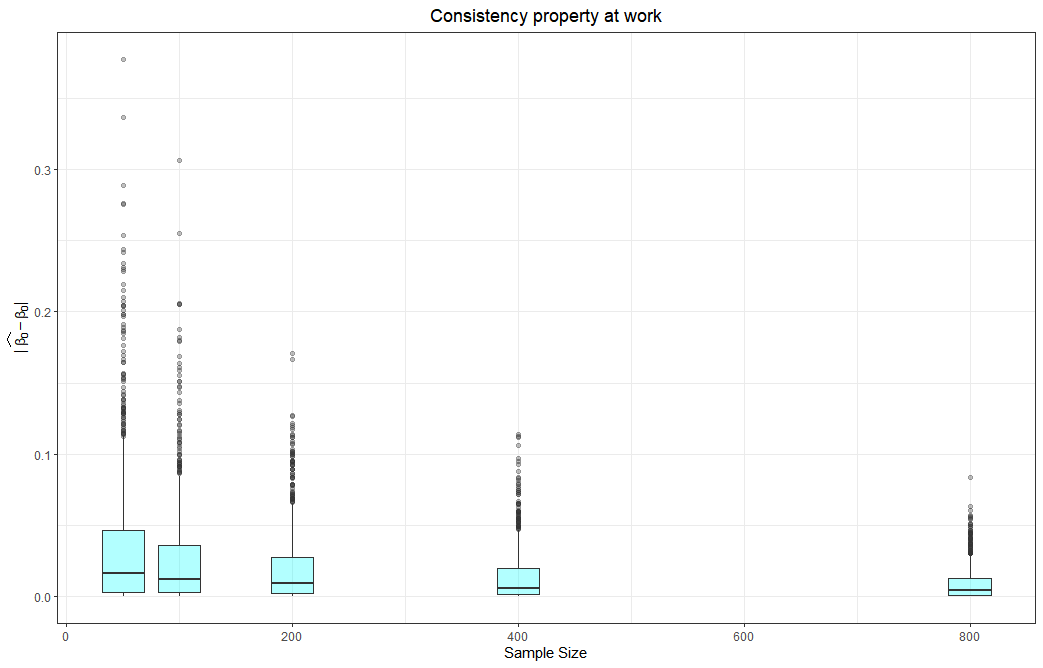
\includegraphics[width = \textwidth]{graphics/samp800n1000b0_box.png}

	%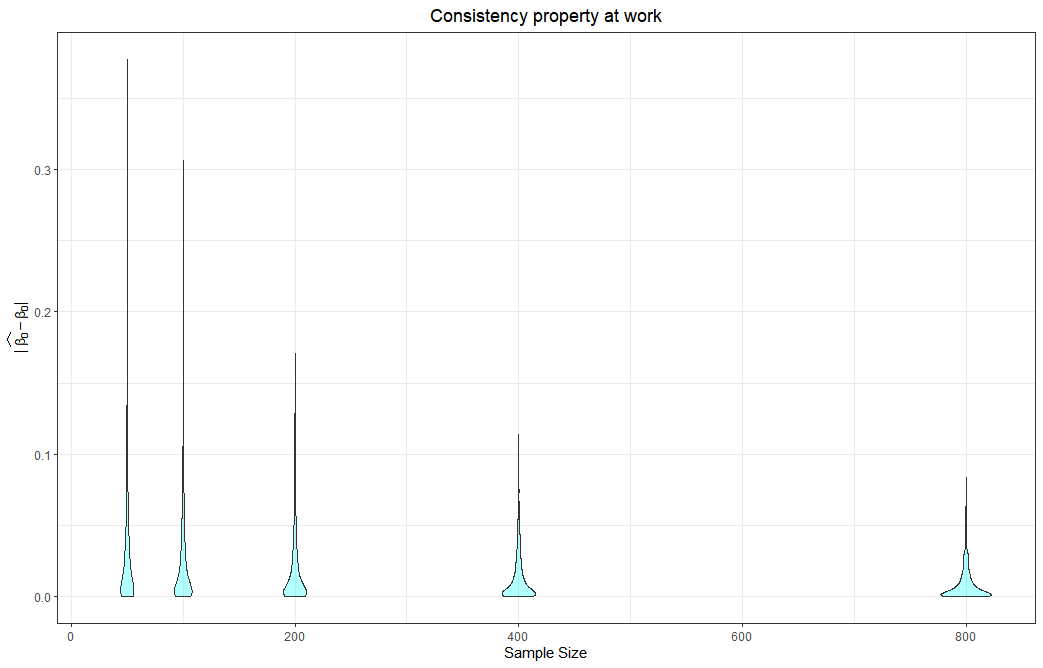
\includegraphics[width = \textwidth]{graphics/samp800n1000b0_violin.png}
\end{center}

\noindent It is almost an identical situation for the $\hat{\beta}_{1}$ estimator as well as $\widehat{\sigma^{2}}$,

\begin{center}
	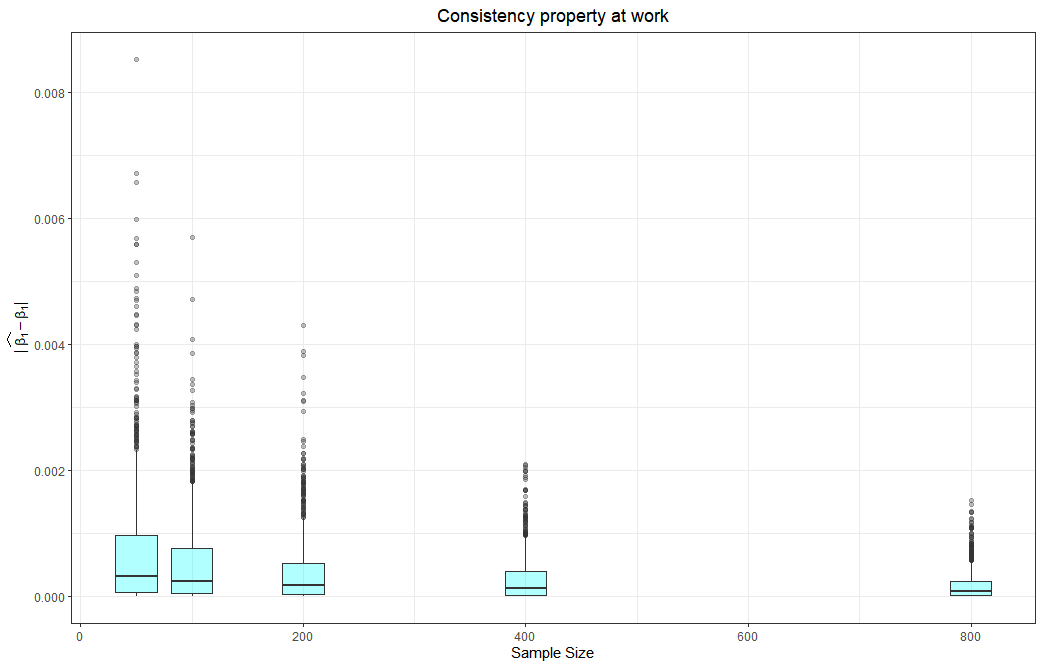
\includegraphics[width = \textwidth]{graphics/samp800n1000b1_box.png}
	%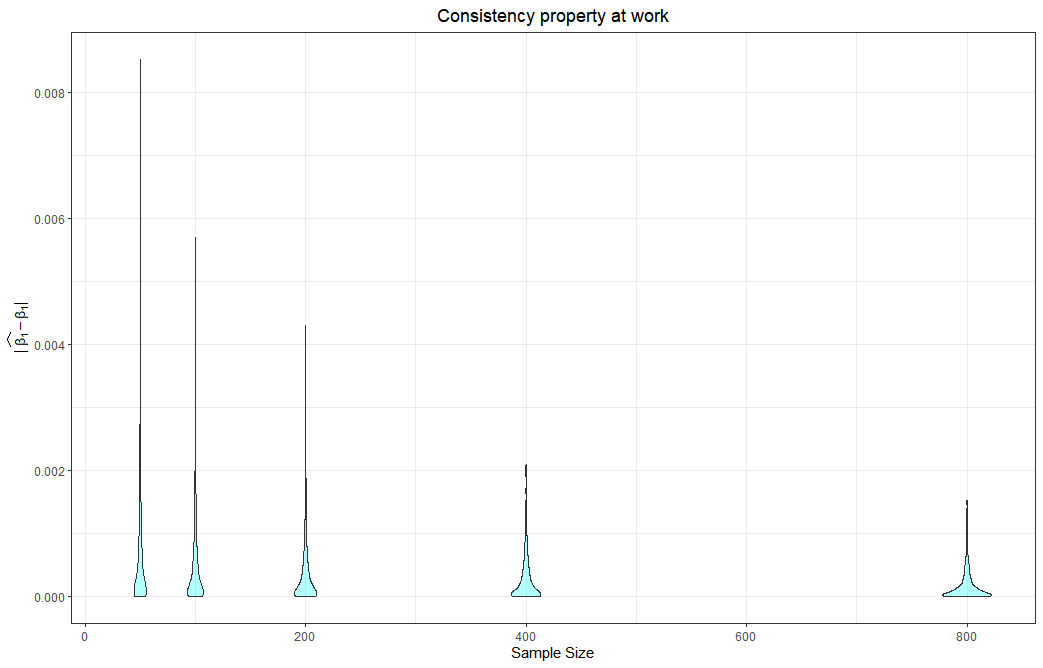
\includegraphics[width = \textwidth]{graphics/samp800n1000b1_violin.png}
	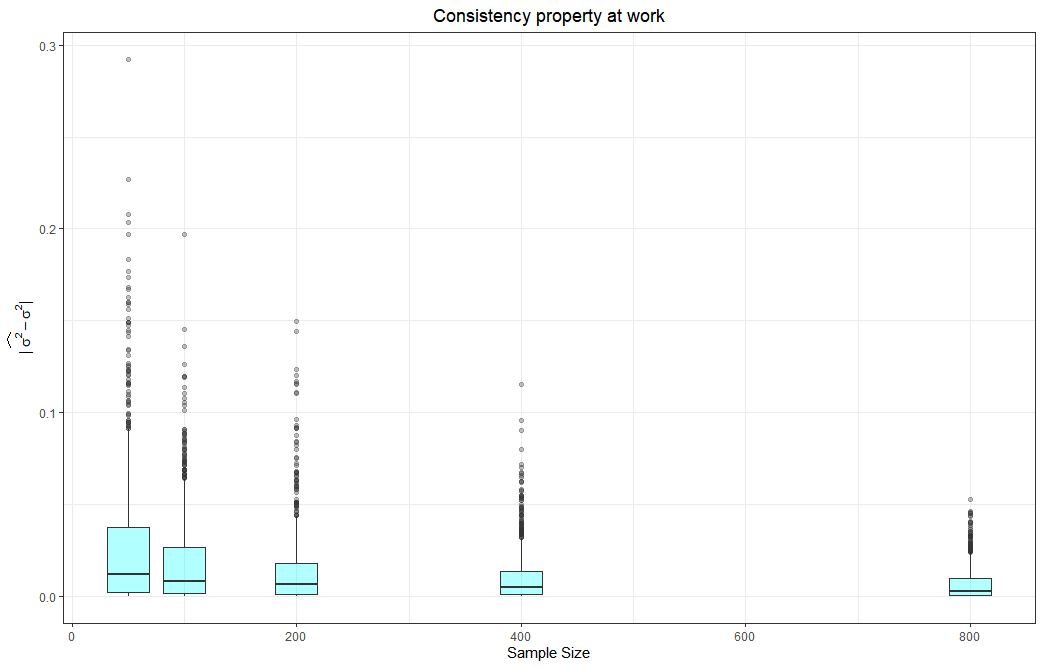
\includegraphics[width = \textwidth]{graphics/samp800n1000sigma_box.png}
	%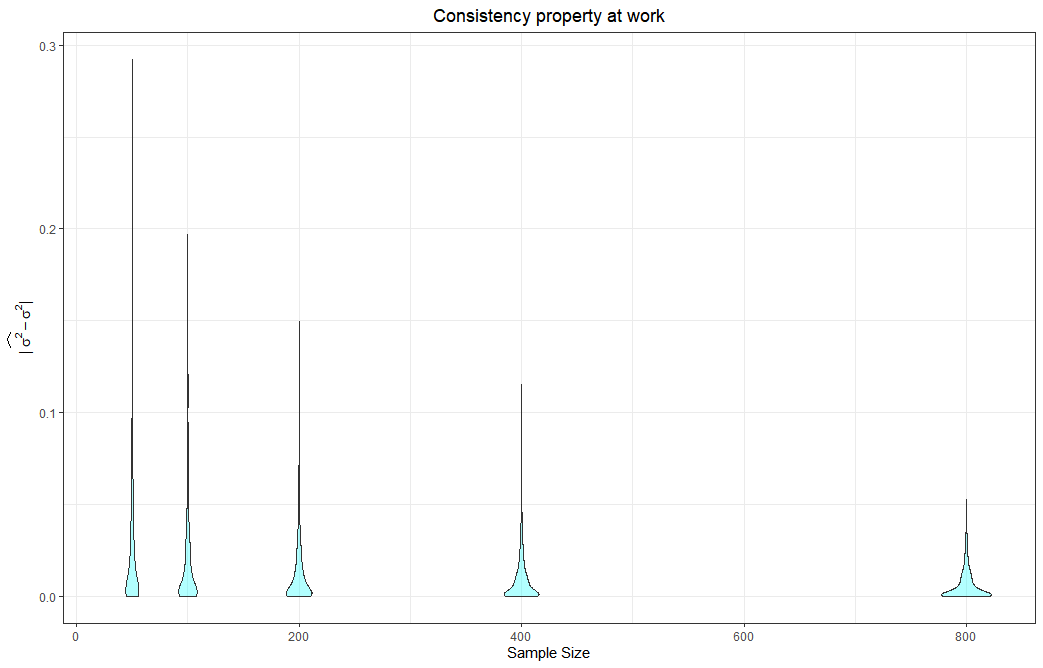
\includegraphics[width = \textwidth]{graphics/samp800n1000sigma_violin.png}
\end{center}
%%%%%%%%%%%%%%%%%%%%%%%%%%%%%%%%%%%%%

\subsubsection{Fisher Information}

To look at the distributional properties of the estimators, we can start by calculating the Fisher information, which measures the sensitivity of the estimates, acting as a way to judge the quality of the estimator. We define $\nabla_{\mathbf{x}}$ to be the gradient, eg $\nabla_{\mathbf{x}} f(\mathbf{x}) = \begin{pmatrix} \frac{\partial f(\mathbf{x}) }{\partial x_{1}} \\ \vdots \\ \frac{\partial f(\mathbf{x}) }{\partial x_{n}} \end{pmatrix}$ where $\mathbf{x} = \begin{pmatrix} x_{1} \\ \vdots \\ x_{n} \end{pmatrix} \in \mathbb{R}^{n}$, because our vector of parameters is size $p+2$, we define the $p+2$ parameter Fisher information by the following,

\begin{align*}
	\mathcal{I}(\ta) &= \E \left( \left( \nabla_{\ta} \LL (\ta) \right) \left( \nabla_{\ta} \LL (\ta) \right)^{T} \right). \numberthis \label{fisherinformation:definition}
\end{align*}

\noindent For simplicity of calculation we wish to show the following result,

\begin{align*}
	-\E \left( \nabla_{\ta}^{2} \LL (\ta) \right) &= \mathcal{I}(\ta). \numberthis \label{fisherinformation:alt}
\end{align*}

\noindent To show this, we begin with a simpler result,

\begin{align*}
	\int_{-\infty}^{\infty} f(\y | \ta) dy &= 1,\\
	\nabla_{\ta} \int_{-\infty}^{\infty} f(\y | \ta) dy &=  \nabla_{\ta}1,\\
	\int_{-\infty}^{\infty} \nabla_{\ta} f(\y | \ta) dy &=  \mathbf{0},\\
	\nabla_{\ta} \int_{-\infty}^{\infty} \nabla_{\ta} f(\y | \ta) dy &=  \nabla_{\ta} \mathbf{0},\\
	\int_{-\infty}^{\infty} \nabla_{\ta}^{2} f(\y | \ta) dy &=  0 \in \mathcal{M}_{\left(p+2\right) \times \left(p+2\right)}. \numberthis \label{useful1}
\end{align*}

\noindent This is a useful result we will apply later on, but to prove the equivalence between \refeq{fisherinformation:definition} and \refeq{fisherinformation:alt} we will begin with the hessian from the latter,

\begin{align*}
	\nabla_{\ta}^{2} \LL (\ta) &= \nabla_{\ta} \left( \nabla_{\ta} \LL (\ta) \right),\\
	&= \nabla_{\ta} \left( \left( \nabla_{\ta} \mathcal{L} (\ta) \right) \mathcal{L}^{-1} (\ta) \right),\\
	&= \left( \nabla_{\ta}^{2} \mathcal{L} (\ta) \right) \mathcal{L}^{-1} (\ta) - \left( \nabla_{\ta} \mathcal{L} (\ta) \right) \left( \nabla_{\ta} \mathcal{L} (\ta) \right)^{T} \mathcal{L}^{-2} (\ta),\\
	-\E \left( \nabla_{\ta}^{2} \LL (\ta) \right) &= -\E \left( \left( \nabla_{\ta}^{2} \mathcal{L} (\ta) \right) \mathcal{L}^{-1} (\ta) - \left( \nabla_{\ta} \mathcal{L} (\ta) \right) \left( \nabla_{\ta} \mathcal{L} (\ta) \right)^{T} \mathcal{L}^{-2} (\ta) \right) ,\\
	&= \E \left( \left( \nabla_{\ta} \mathcal{L} (\ta) \right) \left( \nabla_{\ta} \mathcal{L} (\ta) \right)^{T} \mathcal{L}^{-2} (\ta) \right) - \E \left( \left( \nabla_{\ta}^{2} \mathcal{L} (\ta) \right) \mathcal{L}^{-1} (\ta) \right),\\
	&= \int_{-\infty}^{\infty} \left( \left( \nabla_{\ta} \mathcal{L} (\ta) \right) \left( \nabla_{\ta} \mathcal{L} (\ta) \right)^{T} \mathcal{L}^{-2} (\ta) \right)f(\y|\ta)dy -\\
	&\hspace{2cm} \int_{-\infty}^{\infty} \left( \left( \nabla_{\ta}^{2} \mathcal{L} (\ta) \right) \mathcal{L}^{-1} (\ta) \right)f(\y|\ta)dy.
\end{align*}

\noindent Here we have to note that $f(y|\ta) = \mathcal{L} (\ta)$ as they are the density and the likelihood of the same distribution, this allows for some simplification,

\begin{align*}
	-\E \left( \nabla_{\ta}^{2} \LL (\ta) \right) &= \int_{-\infty}^{\infty} \left( \nabla_{\ta} \mathcal{L} (\ta)\mathcal{L}^{-1} (\ta) \right) \left( \nabla_{\ta} \mathcal{L} (\ta) \mathcal{L}^{-1} (\ta)\right)^{T} f(\y|\ta)dy -\\
	&\hspace{2cm} \int_{-\infty}^{\infty}  \nabla_{\ta}^{2} \mathcal{L} (\ta)dy,\\
	&= \int_{-\infty}^{\infty} \left( \nabla_{\ta} \LL (\ta) \right) \left( \nabla_{\ta} \LL (\ta) \right)^{T}  f(\y|\ta)dy -\\
	&\hspace{2cm} \int_{-\infty}^{\infty} \nabla_{\ta}^{2} f(\y|\ta) dy.
\end{align*}

\noindent Using \refeq{useful1}, and reverting the integral back into an expectation,

\begin{align*}
	-\E \left( \nabla_{\ta}^{2} \LL (\ta) \right) &= \E \left( \left( \nabla_{\ta} \LL (\ta) \right) \left( \nabla_{\ta} \LL (\ta) \right)^{T}  \right) - 0,\\
	&= \mathcal{I} (\ta).
\end{align*}

With that proven, we can calculate the Fisher information for the maximum likelihood estimates,

\begin{align*}
	\mathcal{I}(\bm{\beta},\sigma^{2}) &= -\E \begin{pmatrix} \frac{\partial^{2}}{\partial \bm{\beta}^{2}}\log{\mathcal{L}} & \frac{\partial^{2}}{\partial \bm{\beta} \partial \sigma^{2}}\log{\mathcal{L}} \\ \frac{\partial^{2}}{\partial \sigma^{2} \partial \bm{\beta}}\log{\mathcal{L}} & \frac{\partial^{2}}{\partial \left(\sigma^{2} \right)^{2}}\log{\mathcal{L}} \end{pmatrix}.
\end{align*}

\noindent Some of parts of this expression we have already calculated earlier, so we will substitute \eqref{partialbeta2} and \eqref{partialsig2}, but we need to derive one more time \eqref{partialbeta1} and \eqref{partialsig1} before substituting those. From \eqref{partialbeta1},

\begin{align*}
	\frac{\partial}{\partial \bm{\beta}}  \log\mathcal{L}(\bm{\beta},\sigma^{2} | \mathbf{y}) &= \frac{1}{\sigma^{2}} \s \mathbf{x}_{i} \left( y_{i} - \mathbf{x}_{i}^{T} \bm{\beta} \right),\\
	\frac{\partial^{2}}{\partial \sigma^{2} \partial \bm{\beta}} \log\mathcal{L}(\bm{\beta},\sigma^{2} | \mathbf{y}) &= -\frac{1}{\left( \sigma^{2} \right)^{2}} \s \mathbf{x}_{i} \left( y_{i} - \mathbf{x}_{i}^{T} \bm{\beta} \right), \\
	&= \frac{\partial^{2}}{\partial \bm{\beta} \partial \sigma^{2}} \log\mathcal{L}(\bm{\beta},\sigma^{2} | \mathbf{y}).
\end{align*}

\noindent So we can construct the Fisher information matrix, 

\begin{align*}
	\mathcal{I}(\bm{\beta},\sigma^{2}) &= -\E \begin{pmatrix} -\frac{1}{\sigma^{2}} \s \mathbf{x}_{i} \mathbf{x}_{i}^{T} & - \frac{1}{\left( \sigma^{2} \right)^{2}} \s \mathbf{x}_{i} \left( y_{i} - \mathbf{x}_{i}^{T} \bm{\beta} \right) \\ -\frac{1}{\left( \sigma^{2} \right)^{2}} \s \mathbf{x}_{i} \left( y_{i} - \mathbf{x}_{i}^{T} \bm{\beta} \right) & \frac{n}{2 \left( \sigma^{2} \right)^{2}} -\frac{1}{\left( \sigma^{2}\right)^{3}} \s \left( y_{i} - \mathbf{x}_{i}^{T} \bm{\beta}\right)^{2} \end{pmatrix},\\
	&= \begin{pmatrix} \frac{1}{\sigma^{2}} \s \mathbf{x}_{i} \mathbf{x}_{i}^{T} & \E \left( \frac{1}{\left( \sigma^{2} \right)^{2}} \s \mathbf{x}_{i} \left( y_{i} - \mathbf{x}_{i}^{T} \bm{\beta} \right) \right) \\ \E \left( \frac{1}{\left( \sigma^{2} \right)^{2}} \s \mathbf{x}_{i} \left( y_{i} - \mathbf{x}_{i}^{T} \bm{\beta} \right) \right) & \E \left( - \frac{n}{2\left( \sigma^{2} \right)^{2}}  + \frac{1}{\left( \sigma^{2}\right)^{3}} \s \left( y_{i} - \mathbf{x}_{i}^{T} \bm{\beta}\right)^{2} \right) \end{pmatrix},\\
	&= \begin{pmatrix} \frac{1}{\sigma^{2}} \s \mathbf{x}_{i} \mathbf{x}_{i}^{T} & \frac{1}{\left( \sigma^{2} \right)^{2}} \s \mathbf{x}_{i} \left( \E \left( y_{i}\right) - \mathbf{x}_{i}^{T} \bm{\beta} \right) \\ \frac{1}{\left( \sigma^{2} \right)^{2}} \s \mathbf{x}_{i} \left( \E \left( y_{i} \right) - \mathbf{x}_{i}^{T} \bm{\beta} \right) & - \frac{n}{2\left( \sigma^{2} \right)^{2}}  + \frac{1}{\left( \sigma^{2}\right)^{3}} \s \E \left( \left( y_{i} - \mathbf{x}_{i}^{T} \bm{\beta}\right)^{2} \right) \end{pmatrix},\\
	&= \begin{pmatrix} \frac{1}{\sigma^{2}} \s \mathbf{x}_{i} \mathbf{x}_{i}^{T} & \frac{1}{\left( \sigma^{2} \right)^{2}} \s \mathbf{x}_{i} \left( \mathbf{x}_{i}^{T} \bm{\beta} - \mathbf{x}_{i}^{T} \bm{\beta} \right) \\ \frac{1}{\left( \sigma^{2} \right)^{2}} \s \mathbf{x}_{i} \left( \mathbf{x}_{i}^{T} \bm{\beta} - \mathbf{x}_{i}^{T} \bm{\beta} \right) & - \frac{n}{2\left( \sigma^{2} \right)^{2}}  + \frac{1}{\left( \sigma^{2}\right)^{3}} \s \left( \sigma^{2} \right) \end{pmatrix},\\
	&= \begin{pmatrix} \frac{1}{\sigma^{2}} \s \mathbf{x}_{i} \mathbf{x}_{i}^{T} &0 \\ 0 & - \frac{n}{2 \left( \sigma^{2} \right)^{2}}  + \frac{n}{\left( \sigma^{2} \right)} \end{pmatrix}.\\
	&= \begin{pmatrix} \frac{1}{\sigma^{2}} \s \mathbf{x}_{i} \mathbf{x}_{i}^{T} &0 \\ 0 & \frac{n}{2 \left( \sigma^{2} \right)^{2}} \end{pmatrix}. \numberthis \label{realfisherinfo}
\end{align*}

\subsubsection{Asymptotic Normality}

We want to also know the distributional properties of $\widehat{\bm{\beta}}$, so we can apply statistical tests to it, find out how it is distributed looking at \refeq{real_beta}, 

\begin{align*}
	\widehat{\bm{\beta}} &= \left( \sum_{i = 1}^{n} \mathbf{x}_{i} \mathbf{x}_{i}^{T} \right)^{-1} \left( \sum_{i = 1}^{n} \mathbf{x}_{i} y_{i}\right).
\end{align*}

\noindent From the right hand side, $y_{i}$ is the only random variable, with the following distribution,

\begin{align*}
	y_{i} \sim \mathcal{N} \left( \mathbf{x}_{i}^{T} \bm{\beta}, \sigma^{2} \right).
\end{align*}

\noindent We can then transform the left hand side using properties of the normal distribution,

\begin{align*}
	\mathbf{x}_{i} y_{i} & \sim \mathcal{N} \left( \mathbf{x}_{i} \mathbf{x}_{i}^{T} \bm{\beta}, \mathbf{x}_{i}\sigma^{2} \mathbf{x}_{i}^{T} \right), \\
	\sum_{i = 1}^{n} \mathbf{x}_{i} y_{i} & \sim \mathcal{N} \left( \sum_{i = 1}^{n} \mathbf{x}_{i} \mathbf{x}_{i}^{T} \bm{\beta}, \sigma^{2} \sum_{i = 1}^{n} \mathbf{x}_{i} \mathbf{x}_{i}^{T} \right), \\
	\left( \sum_{i = 1}^{n} \mathbf{x}_{i} \mathbf{x}_{i}^{T} \right)^{-1} \left( \sum_{i = 1}^{n} \mathbf{x}_{i} y_{i} \right) & \sim \mathcal{N} \left(  \bm{\beta} , \sigma^{2} \left( \sum_{i = 1}^{n} \mathbf{x}_{i} \mathbf{x}_{i}^{T} \right)^{-1} \right), \\
	\widehat{\bm{\beta}} & \sim \mathcal{N} \left(  \bm{\beta} , \sigma^{2} \left( \sum_{i = 1}^{n} \mathbf{x}_{i} \mathbf{x}_{i}^{T} \right)^{-1} \right).
\end{align*}

We see that the covariance here does coincide with the well known result that the variance of the parameter is the inverse $\bm{\beta}$ term of the fisher information in \refeq{realfisherinfo}.

\begin{align*}
	\widehat{\bm{\beta}} - \bm{\beta} &\sim \mathcal{N} \left( \mathbf{0}, \sigma^{2} \left( \sum_{i = 1}^{n} \mathbf{x}_{i} \mathbf{x}_{i}^{T} \right)^{-1} \right), \\
	\frac{1}{\sigma} \left( \sum_{i = 1}^{n} \mathbf{x}_{i} \mathbf{x}_{i}^{T} \right)^{\frac{1}{2}} \left( \widehat{\bm{\beta}} - \bm{\beta} \right) &\sim \mathcal{N} \left( \mathbf{0}, \mathbb{1}_{p} \right).
\end{align*}

\noindent This is for a known $\sigma^{2}$, we'll leave it here, as to parallel with our findings in the complex regression case, as we do not deal with the distribution of the estimate for the covariance there.

\chapter{Complex Numbered Regression Model}

\section{Complex Model}

Now we seek to construct the complex number model, find out how to estimators look like and observe their properties. Making the move over from the real scenario, our observations become complex along with the data and errors, complex meaning they have the form $a+jb$ where $j$ is the complex number $\sqrt{-1}$. Ultimately for the $i$-th observation out of $n$, our underlying model will look like,

\begin{align*}
	Z_{i} &= \mathbf{x}_{i}^{T}\bm{\beta} + \epsilon_{i}.
\end{align*}

\noindent Where the complex vector $\mathbf{x}_{i} = \left( 1, x_{i1},  \hdots , x_{ip} \right)^{T}$ and $\bm{\beta} = \left( \beta_{0}, \beta_{1},  \hdots,  \beta_{p}\right)^{T}$. However to follow Definition 1 from Ducharme \cite{ducharme2016} we will augment our model, not removing anything, but only adding conjugates of each of the parameters so we can use the nice form of the density, our model for each observations becomes,

\begin{align*}
	\utilde{Z}_{i} &= \utilde{x}_{i} \utilde{\bm{\beta}} + \utilde{\epsilon}_{i}. \numberthis \label{complexmodel}
\end{align*}

\noindent And the full model with $n$ observations,

\begin{align*}
	\utilde{\mathbf{Z}} &= \utilde{X} \utilde{\bm{\beta}} + \utilde{\bm{\epsilon}}. \numberthis \label{complexmodelfull}
\end{align*}

\noindent There is a lot of notation here to unpack and we'll go through them sequentially. Firstly we let $z$ be a complex random variable, so $\mathbf{z}$ is a complex vector, with $\mathbf{z}^{*}$ denoting the conjugate of that vector and $\mathbf{z}^{\ct} = \left( \mathbf{z}^{*} \right)^{T} = \left( \mathbf{z}^{T} \right)^{*}$ to denote the complex conjugate transpose of $\mathbf{z}$. \par
\noindent We then define $\utilde{z}_{i} = \left( z_{i}, z_{i}^{*} \right)^{T}$, a sort of stacked complex vector, different from stacking the real parts and imaginary parts of a complex vector \cite{yan2012}. Then when we put this in vector form we obtain, $\augz = \left( z_{1}, z_{1}^{*}, \hdots, z_{n}, z_{n}^{*} \right)^{T}$. \par
\noindent Almost similarly we can define this stacking operator for a matrix $X$, first we look a single data point $x_{i} = \left( 1, x_{i1}, \dots, x_{ip}\right)^{T}$, when stacked this becomes,

\begin{align*}
	\utilde{x_{i}} &= \begin{pmatrix}
		1 & x_{i1} & \hdots & x_{ip} & 0 & 0 & \hdots & 0\\
		0 & 0 & \hdots & 0 & 1 & x_{i1}^{*} & \hdots & x_{ip}^{*} \\
	\end{pmatrix}.
\end{align*}

\noindent Then for the full matrix of data,

\begin{align*}
	\utilde{X} &= \begin{pmatrix}
		1 & x_{11} & \hdots & x_{1p} & 0 & 0 & \hdots & 0\\
		0 & 0 & \hdots & 0 & 1 & x_{11}^{*} & \hdots & x_{1p}^{*} \\
		\vdots & \vdots & \ddots & \vdots & \vdots & \vdots & \ddots & \vdots \\
		1 & x_{n1} & \hdots & x_{np} & 0 & 0 & \hdots & 0\\
		0 & 0 & \hdots & 0 & 1 & x_{n1}^{*} & \hdots & x_{np}^{*} \\
	\end{pmatrix}.
\end{align*}

\noindent This looks like a mess, although it is, when you take in consideration that the vector of regression parameters $\augb$ will look like $\augb = \left( \beta_{0}, \hdots, \beta_{p}, \beta_{0}^{*}, \hdots, \beta_{p}^{*} \right)^{T}$, an expression like $\left( \utilde{z}_{i} - \utilde{x}_{i} \augb \right)$ makes sense.

%%%%%%%%%%%%%%%%%%%%%%%%%%%%%%%%%%%%%

\subsection{Assumptions}

Different model means different assumptions that need to be made, the assumptions would mostly be clear and similar to the real case.
\begin{itemize}
	\item Each augmented pair of errors are independent and identically distributed complex improper normal with $0$ mean and $2$ by $2$ covariance matrix $\Gamma$ which we will get into in a later subsection. Eg $\epsilon_{i} \sim \mathcal{CN} (0,\Gamma)$.
	\item All these parameters in model \refeq{complexmodel} are complex, eg random observations $Z_{i}$, data vector $\mathbf{x}_{i}$, regression parameter $\bm{\beta}$ and the error $\epsilon_{i}$ are all complex.
	\item There is a linear relationship between the observation $Z_{i}$ and the data $\mathbf{x}_{i}$.
\end{itemize}

%%%%%%%%%%%%%%%%%%%%%%%%%%%%%%%%%%%%%

\subsection{Improper Complex Normal Distribution}

We will mostly use the notation borrowed from the Ducharme paper \cite{ducharme2016} however changing one or two things to suit our needs. One way to look at complex normal random variables, is that the real and imaginary parts of $Z$ are from some normal distribution and that there is also some correlation between the two parts. So each observation $Z_{i} = \Chi_{1} + j \Chi_{2}$ is really from a two dimensional multivariate normal,

\begin{align*}
	\bm{\Chi} = (\Chi_{1}, \Chi_{2})^{T} \sim \mathcal{N}_{2} (\bm{\mu}_{\Chi}, \Sigma_{\Chi}).
\end{align*}

\noindent Where $\Sigma_{\Chi}$ is a positive definite covariance matrix. A transformation can be made from $\bm{\Chi}$ to $\utilde{Z}_{i}$ using a handy matrix found in both \cite{ducharme2016} and \cite{picinobo1998},

\begin{align*}
	M = \frac{1}{2} \begin{pmatrix}
		\mathbb{1}_{n} & \mathbb{1}_{n} \\
		-j \mathbb{1}_{n} & j \mathbb{1}_{n}
	\end{pmatrix}&, \hspace{1cm}
	M^{-1} = \begin{pmatrix}
		\mathbb{1}_{n} & j \mathbb{1}_{n} \\
		\mathbb{1}_{n} & -j \mathbb{1}_{n}
	\end{pmatrix}  = 2 M^{\ct},\\
	\bm{\Chi} &= M \utilde{Z}_{i} = M \begin{pmatrix} Z_{i} \\ Z_{i}^{*} \end{pmatrix}.
\end{align*}

\noindent Here the $\mathbb{1}_{n}$ denotes the identity matrix of size $n$, and $n$ in this case is $1$. We can then use this matrix to show a relationship between $\Sigma_{\Chi}$ and $\Gamma$, $\Gamma$ which we will define as,

\begin{align*}
	\Gamma &= \E \left[ \utilde{\epsilon}_{i} \utilde{\epsilon}_{i}^{\ct}\right], \\
	&=\E \left[ 
		\begin{pmatrix}
			\epsilon_{i} \\
			\epsilon_{i}^{*}
		\end{pmatrix}
		\begin{pmatrix}
			\epsilon_{i} \\
			\epsilon_{i}^{*}
		\end{pmatrix}^{\ct}
	\right], \\
	&= \begin{pmatrix}
		\E \left[
			\epsilon_{i} \epsilon_{i}^{*}
		\right] &
		\E \left[
			\epsilon_{i} \epsilon_{i}
		\right] \\
		\E \left[
			\epsilon_{i}^{*} \epsilon_{i}^{*}
		\right] &
		\E \left[
			\epsilon_{i}^{*} \epsilon_{i}
		\right]
	\end{pmatrix}, \numberthis \label{complexcovarianceexpanded}\\
	&= \begin{pmatrix}
	K & J \\
	J^{*} &  K
	\end{pmatrix}. \numberthis \label{complexcovariancejk}
\end{align*}

\noindent On a side, we can get complex valued $J$, however $K$ is always real valued. Commonly $K$ is referred to as the covariance and $J$ is called pseudo-covariance, in the proper complex normal distribution $J$ is set to $0$, hence we use the improper complex normal to add some level of generalisation and capture more information that might otherwise be left out of the proper complex normal distribution. \par
\noindent This also means that $\Gamma$ is a $2$ by $2$ matrix, however when considering an augmented vector of $\utilde{\mathbf{z}} = (z_{1},  z_{1}^{*}, ..., z_{n}, z_{n}^{*})^{T}$, $\Gamma$ will be block diagonal matrix with it's 2 by 2 self as the blocks and in another case if $\utilde{\mathbf{z}} = (\mathbf{z}^{T}, \mathbf{z}^{*T})^{T}$ then the $2n$ by $2n$ matrix $\Gamma$ using the notation in \refeq{complexcovariancejk} will be in weird form, $K$'s on the main diagonal and $J$'s on the $n$-th super-diagonal and $J^{*}$'s on the $n$-th sub-diagonal, here's an illustration to better explain,

\begin{align*} 
	\Gamma &= \begin{bmatrix}
		K \mathbb{1}_{n} & J \mathbb{1}_{n} \\
		J^{*} \mathbb{1}_{n} & K \mathbb{1}_{n}
	\end{bmatrix}.
\end{align*}

\noindent This was not super important, but the notation used for the three different $\Gamma$ will not be differentiated, because generally they are dependent on circumstance and their meanings are similar and are all hermitian. Moving on from this digression, the relationship between $\Sigma_{\Chi}$ and $\Gamma$, taking the $M$ matrix with n = 1 and the \refeq{complexcovarianceexpanded} definition of $\Gamma$ ( 2 by 2),

\begin{align*}
	M \Gamma M^{\ct} &= \frac{1}{4} \begin{pmatrix}
		1 & 1 \\
		- j & j
	\end{pmatrix}
	\begin{pmatrix}
		\E \left[
			\epsilon_{i} \epsilon_{i}^{*}
		\right] &
		\E \left[
			\epsilon_{i} \epsilon_{i}
		\right] \\
		\E \left[
			\epsilon_{i}^{*} \epsilon_{i}^{*}
		\right] &
		\E \left[
			\epsilon_{i}^{*} \epsilon_{i}
		\right]
	\end{pmatrix}
	\begin{pmatrix}
		1 & j \\
		1 & - j 
	\end{pmatrix},\\
	&= \frac{1}{4} \left( \begin{matrix}
		\E \left[
		    \epsilon_{i} \epsilon_{i}^{*}
		\right] + 
		\E \left[
		    \epsilon_{i} \epsilon_{i}
		\right] + 
		\E \left[
		    \epsilon_{i}^{*} \epsilon_{i}^{*}
		\right] +
		\E \left[
		    \epsilon_{i}^{*} \epsilon_{i}
		\right] \\
		- j \E \left[
		    \epsilon_{i} \epsilon_{i}^{*}
		\right] + 
		j \E \left[
		    \epsilon_{i} \epsilon_{i}
		\right] - 
		j \E \left[
		    \epsilon_{i}^{*} \epsilon_{i}^{*}
		\right] +
		j \E \left[
		    \epsilon_{i}^{*} \epsilon_{i}
		\right]
		\end{matrix}\right.\\
		&\qquad \qquad \qquad \qquad \left. \begin{matrix}
		j \E \left[
		    \epsilon_{i} \epsilon_{i}
		\right] - 
		j \E \left[
		    \epsilon_{i} \epsilon_{i}^{*}
		\right] + 
		j \E \left[
		    \epsilon_{i}^{*} \epsilon_{i}^{*}
		\right] -
		j \E \left[
		    \epsilon_{i}^{*} \epsilon_{i}
		\right] \\
		\E \left[
		    \epsilon_{i} \epsilon_{i}^{*}
		\right] -
		\E \left[
		    \epsilon_{i} \epsilon_{i}
		\right] -
		\E \left[
		    \epsilon_{i}^{*} \epsilon_{i}^{*}
		\right] +
		\E \left[
		    \epsilon_{i}^{*} \epsilon_{i}
		\right]
	\end{matrix} \right).
\end{align*}

\noindent This mess here, in-fact can be simplified, first by taking a look at the three different expectations and using $\epsilon_{i} = \text{Re} \left( \epsilon_{i} \right) + j \text{Im} \left( \epsilon_{i} \right)$, the expectations can be written as,

\begin{align*}
    \E \left[ \epsilon_{i} \epsilon_{i} \right] &= \E \left[ \text{Re} ( \epsilon_{i} )^{2} \right] + 2 j \E \left[ \text{Re} ( \epsilon_{i} ) \text{Im} ( \epsilon_{i} ) \right] - \E \left[ \text{Im} ( \epsilon_{i} )^{2} \right],\\
    \E \left[ \epsilon_{i}^{*} \epsilon_{i}^{*} \right] &= \E \left[ \text{Re} ( \epsilon_{i} )^{2} \right] - 2 j \E \left[ \text{Re} ( \epsilon_{i} ) \text{Im} ( \epsilon_{i} ) \right] - \E \left[ \text{Im} ( \epsilon_{i} )^{2} \right],\\
    \E \left[ \epsilon_{i}^{*} \epsilon_{i} \right] = \E \left[ \epsilon_{i} \epsilon_{i}^{*} \right] &= \E \left[ \text{Re} ( \epsilon_{i} )^{2} \right] + \E \left[ \text{Im} ( \epsilon_{i} )^{2} \right].
\end{align*}

\noindent We can this substitute all these into the $M \Gamma M^{\ct}$ matrix multiplication, netting the very nice result,

\begin{align*}
	M \Gamma M^{\ct} &= 
	\begin{pmatrix} 
		\E \left[ \text{Re} ( \epsilon_{i} )^{2} \right] & \E \left[ \text{Re} ( \epsilon_{i} ) \text{Im} ( \epsilon_{i} ) \right] \\
		\E \left[ \text{Re} ( \epsilon_{i} ) \text{Im} ( \epsilon_{i} ) \right] & \E \left[ \text{Im} ( \epsilon_{i} )^{2} \right]
	\end{pmatrix}, \\
	M \Gamma M^{\ct} &= \Sigma_{\Chi}. \numberthis \label{MVTN_CN_cov}
\end{align*}

\noindent As this is the definition of the multivariate covariance, as $\Chi_{1}$ and $\Chi_{2}$ are the pair of random variables with variances $\text{Re} ( \epsilon_{i} )$ and $\text{Im} ( \epsilon_{i} )$ respectively. This result also leads to the following conclusions, using Leibniz Formula for determinants midway,

\begin{align*}
	| \Sigma_{\Chi} | &= | M \Gamma M^{\ct} |,\\
	&= | M | \cdot | \Gamma | \cdot | M^{\ct} |,\\
	&= \left| \frac{1}{2} 
		\begin{pmatrix}
			\mathbb{1}_{n} & \mathbb{1}_{n} \\
			- j \mathbb{1}_{n} & j \mathbb{1}_{n}
		\end{pmatrix}
		\right| \cdot
		| \Gamma | \cdot
		\left| \frac{1}{2} 
		\begin{pmatrix}
			\mathbb{1}_{n} & j \mathbb{1}_{n} \\
			\mathbb{1}_{n} & - j \mathbb{1}_{n}
		\end{pmatrix}
		\right|,\\
	&= 2^{- 2 n} 
		\left| \mathbb{1}_{n} - \mathbb{1}_{n} \left( j \mathbb{1}_{n} \right)^{-1} \left( - j \mathbb{1}_{n} \right) \right| \cdot
		| j \mathbb{1}_{n} | \cdot
		| \Gamma | \\
	&\hspace{2cm} \cdot 2^{- 2 n} \cdot
		\left| \mathbb{1}_{n} - j \mathbb{1}_{n} \left( - j \mathbb{1}_{n} \right)^{-1} \mathbb{1}_{n} \right| \cdot
		\left| - j \mathbb{1}_{n} \right|, \\
	&= 2^{- 2 n} \cdot
		\left| \mathbb{1}_{n} + \mathbb{1}_{n} \right| \cdot
		j^{n} \cdot
		| \Gamma | \cdot
		2^{- 2 n} \cdot
		\left| \mathbb{1}_{n} + \mathbb{1}_{n} \right| \cdot
		\left( - j \right)^{n},\\
	&= 2^{- 2 n} \cdot 2^{n} \cdot j^{n} \cdot | \Gamma | \cdot 2^{- 2 n} \cdot 2^{n} \cdot \left( - j \right)^{n},\\
	&= 2^{- 2 n} \cdot | \Gamma |.
\end{align*}

And since $\Gamma$ and $\Sigma_{\Chi}$ are positive definite, they are invertible,

\begin{align*}
	\Sigma_{\Chi}^{-1} &= \left( M \Gamma M^{\ct} \right)^{-1},\\
	&= M^{-1 \ct} \Gamma^{-1} M^{-1},\\
	&= 4 M \Gamma^{-1} M^{\ct}.
\end{align*}

\noindent With these nice relations that can be generalised to the $2n$-th dimension, we can look at rewriting the multivariate normal density, suppose $\bm{\Chi} \sim \mathcal{N}_{2n} \left( \bm{\mu}_{\Chi}, \Sigma_{\Chi} \right)$, recall that $\mathbf{x} = M \utilde{\mathbf{z}}$ and we'll denote $\E \left[ \utilde{\mathbf{z}} \right] = \utilde{\bm{\mu}}$, so $\bm{\mu}_{\Chi} = M \utilde{\bm{\mu}}$,

\begin{align*}
	f_{\Chi} ( \mathbf{x} ) &= \frac{1}{ \left( 2 \pi \right)^{n} | \Sigma_{\Chi} |^{\frac{1}{2}}} \exp{ \left( -\frac{1}{2} \left( \mathbf{x} - \bm{\mu}_{\Chi} \right)^{T} \Sigma_{\Chi}^{-1} \left( \mathbf{x} - \bm{\mu}_{\Chi} \right) \right) },\\
	&= \frac{1}{\left( 2 \pi \right)^{n} \left( 2^{- 2 n } |\Gamma| \right)^{ \frac{1}{2} } } \exp{ \left( -\frac{1}{2} \left( \mathbf{x} - \bm{\mu}_{\Chi} \right)^{T} M^{-1 \ct} \Gamma^{-1} M^{-1} \left( \mathbf{x} - \bm{\mu}_{\Chi} \right) \right) },\\
	&= \frac{1}{\pi^{n}|\Gamma|^{ \frac{1}{2} } } \exp{ \left( -\frac{1}{2} \left( M^{-1 * } \mathbf{x}^{*} - M^{-1 * } \bm{\mu}_{\Chi}^{*} \right)^{T} \Gamma^{-1} \left( M^{-1} \mathbf{x} - M^{-1} \bm{\mu}_{\Chi} \right) \right) },\\
	f_{Z} ( \mathbf{z} ) &= \frac{1}{\pi^{n}|\Gamma|^{ \frac{1}{2} } } \exp{ \left( -\frac{1}{2} \left( \utilde{\mathbf{z}}^{*} - \utilde{\bm{\mu}}^{*} \right)^{T} \Gamma^{-1} \left( \utilde{\mathbf{z}} - \utilde{\bm{\mu}} \right) \right) },\\
	f_{Z} ( \mathbf{z} ) &= \frac{1}{\pi^{n}|\Gamma|^{ \frac{1}{2} } } \exp{ \left( -\frac{1}{2} \left( \utilde{\mathbf{z}} - \utilde{\bm{\mu}} \right)^{\ct} \Gamma^{-1} \left( \utilde{\mathbf{z}} - \utilde{\bm{\mu}} \right) \right) }.
\end{align*}

\noindent Which leads us to the definition of the complex normal distribution where $Z \sim \mathcal{CN}_{n} \left( \bm{\mu}, \Gamma \right)$. \par
So in the case of our complex model which has observations that are $Z$ with mean $X \bm{\beta}$, it is distributed $Z \sim \mathcal{CN}_{n} \left( \bm{\mu}, \Gamma \right)$ with a density of,

\begin{align*}
	f_{Z} ( \mathbf{z} ) &= \frac{1}{\pi^{n}|\Gamma|^{ \frac{1}{2} } } \exp{ \left( -\frac{1}{2} \left( \utilde{\mathbf{z}} - \utilde{X} \utilde{\bm{\beta}} \right)^{\ct} \Gamma^{-1} \left( \utilde{\mathbf{z}} - \utilde{X} \utilde{\bm{\beta}} \right) \right) }
\end{align*}

\noindent Then for each observation $Z_{i} \sim \mathcal{CN} \left( x_{i} \bm{\beta}, \Gamma \right)$

\begin{align*}
f_{Z_{i}} (z_{i}) = \frac{1}{\pi |\Gamma|^{\frac{1}{2}}} \exp{ \left( - \frac{1}{2} \left( \utilde{z}_{i} - \utilde{x}_{i} \augb \right)^{\ct} \Gamma^{-1} \left( \utilde{z}_{i} - \utilde{x}_{i} \augb \right) \right)}. \numberthis \label{modeldistribution}
\end{align*}

\noindent Since each of the $\epsilon_{i}$ were independent, so are the $z_{i}$, this will be helpful for analytically solving the likelihood.

%%%%%%%%%%%%%%%%%%%%%%%%%%%%%%%%%%%%%

\subsection{Likelihood}

The next step to obtaining estimators for parameters in our model is to formulate the likelihood, we shall use a simplification to help ease notation letting $\ta = \left( \augb, \augb^{*}, \Gamma \right)$.

\begin{align*}
	\mathcal{L} (\ta) &= f_{\mathbf{Z}}(\mathbf{z} | \ta),\\
	&= \prod_{i=1}^{n} f_{Z_{i}}(z_{i} | \ta),\\
	&= \prod_{i=1}^{n} \left( \frac{1}{\pi |\Gamma|^{\frac{1}{2}}} \exp{ \left( - \frac{1}{2}\left( \utilde{z}_{i} - \utilde{x}_{i} \augb \right)^{\ct} \Gamma^{-1} \left( \utilde{z}_{i} - \utilde{x}_{i} \augb \right) \right)} \right) .
\end{align*}

\noindent Since this is a distribution, we needn't worry about taking the log of the likelihood since it is real,

\begin{align*}
\log{ \mathcal{L} (\ta) } &= \log{ \prod_{i=1}^{n} \left( \frac{1}{\pi |\Gamma|^{\frac{1}{2}}} \exp{ \left( - \frac{1}{2}\left( \utilde{z}_{i} - \utilde{x}_{i} \augb \right)^{\ct} \Gamma^{-1} \left( \utilde{z}_{i} - \utilde{x}_{i} \augb \right) \right)} \right) },\\
\log{ \mathcal{L} (\ta) } &= - n \log{ \left( \pi |\Gamma|^{\frac{1}{2}} \right) } - \frac{1}{2} \sum_{i=1}^{n} \left( \utilde{z}_{i} - \utilde{x}_{i} \augb \right)^{\ct} \Gamma^{-1} \left( \utilde{z}_{i} - \utilde{x}_{i} \augb \right). \numberthis \label{complexloglikelihood}
\end{align*}

\noindent Now we can get maximising and obtaining maximum likelihood estimates.

%%%%%%%%%%%%%%%%%%%%%%%%%%%%%%%%%%%%%

\section{Estimators}

\subsection{Derivation}

\indent Calculation of the estimators involves complex vector calculus specifically the following identities \cite{fischer2002}, where we take $\mathbf{z}$ to be the complex vector variable, $\mathbf{c}$ to be a constant vector, $\mathbf{z}^{*}$ to denote the complex conjugate of $\mathbf{z}$ and $\mathbf{c}^{T}$ to be the transpose of $\mathbf{c}$.

\begin{align}\label{complexvectorcalculus}
	\begin{split}
		\frac{\partial}{\partial \mathbf{z}}\mathbf{c}^{T}\mathbf{z} &= \mathbf{c},\\
		\frac{\partial}{\partial \mathbf{z}^{*}}\mathbf{c}^{T}\mathbf{z} &= \mathbf{0},
	\end{split}
	\begin{split}
		 \frac{\partial}{\partial \mathbf{z}} \mathbf{c}^{T}\mathbf{z}^{*}&=\mathbf{0},\\
		 \frac{\partial}{\partial \mathbf{z}^{*}} \mathbf{c}^{T}\mathbf{z}^{*}&=\mathbf{c}.
	\end{split}
\end{align}

\noindent We can then proceed to differentiate the log-likelihood with respect to our complex vector,

\begin{align*}
	\log{\mathcal{L}(\ta)} &= - n \log{ \left( \pi |\Gamma|^{\frac{1}{2}} \right) } - \frac{1}{2} \sum_{i=1}^{n} \left( \utilde{z}_{i} - \utilde{x}_{i} \augb \right)^{\ct} \Gamma^{-1} \left( \utilde{z}_{i} - \utilde{x}_{i} \augb \right),\\
	\frac{\partial}{\partial \augb} \log{\mathcal{L}(\ta)} &=  \frac{\partial}{\partial \augb} \left( - n \log{ \left( \pi |\Gamma|^{\frac{1}{2}} \right) } - \frac{1}{2} \sum_{i=1}^{n} \left( \utilde{z}_{i} - \utilde{x}_{i} \augb \right)^{\ct} \Gamma^{-1} \left( \utilde{z}_{i} - \utilde{x}_{i} \augb \right) \right),\\
	&= - \mathbf{0} - \frac{1}{2} \cdot \frac{\partial}{\partial \augb} \left( \sum_{i=1}^{n} \left( \utilde{z}_{i} - \utilde{x}_{i} \augb \right)^{\ct} \Gamma^{-1} \left( \utilde{z}_{i} - \utilde{x}_{i} \augb \right) \right),\\
	&= - \frac{1}{2}\sum_{i=1}^{n} \frac{\partial}{\partial \augb} \left( \utilde{z}_{i}^{\ct} \Gamma^{-1} \utilde{z}_{i} - \utilde{z}_{i}^{\ct} \Gamma^{-1} \utilde{x}_{i} \augb - \augb^{\ct} \utilde{x}_{i}^{\ct} \Gamma^{-1} \utilde{z}_{i} + \augb^{\ct} \utilde{x}_{i}^{\ct} \Gamma^{-1} \utilde{x}_{i} \augb \right),\\
	&= - \frac{1}{2} \sum_{i=1}^{n} \frac{\partial}{\partial \augb} \left( \utilde{z}_{i}^{\ct} \Gamma^{-1} \utilde{z}_{i} \right)  + \frac{1}{2} \sum_{i=1}^{n} \frac{\partial}{\partial \augb} \left(\utilde{z}_{i}^{\ct} \Gamma^{-1} \utilde{x}_{i} \augb \right)  \\
	&\hspace{2cm} + \frac{1}{2} \sum_{i=1}^{n} \frac{\partial}{\partial \augb} \left(  \augb^{\ct} \utilde{x}_{i}^{\ct}\Gamma^{-1} \utilde{z}_{i} \right) - \frac{1}{2} \sum_{i=1}^{n} \frac{\partial}{\partial \augb} \left( \augb^{\ct} \utilde{x}_{i}^{\ct} \Gamma^{-1} \utilde{x}_{i} \augb \right),\\
	&= - \mathbf{0} + \frac{1}{2} \sum_{i=1}^{n} \frac{\partial}{\partial \augb} \left( \left( \utilde{x}_{i}^{T} \left( \Gamma^{-1} \right)^{T} \utilde{z}_{i}^{*} \right)^{T} \augb \right)  + \frac{1}{2} \sum_{i=1}^{n} \frac{\partial}{\partial \augb} \left(  \augb^{\ct} \utilde{x}_{i}^{\ct}\Gamma^{-1} \utilde{z}_{i} \right) \\
	&\hspace{2cm}- \frac{1}{2} \sum_{i=1}^{n} \frac{\partial}{\partial \augb} \left( \left( \utilde{x}_{i}^{T} \left( \Gamma^{-1} \right)^{T} \utilde{x}_{i}^{*} \augb^{*} \right)^{T} \augb \right).
\end{align*}

\noindent Using \refeq{complexvectorcalculus}, when differentiating with respect to $\augb$ we keep $\augb^{*}$ constant,

\begin{align*}
	\frac{\partial}{\partial \augb} \log{\mathcal{L}(\ta)} &= \frac{1}{2} \sum_{i=1}^{n} \left(  \utilde{x}_{i}^{T} \left( \Gamma^{-1} \right)^{T} \utilde{z}_{i}^{*} \right) + \mathbf{0} - \frac{1}{2} \sum_{i=1}^{n} \left(  \utilde{x}_{i}^{T} \left( \Gamma^{-1} \right)^{T} \utilde{x}_{i}^{*} \augb^{*} \right).
\end{align*}

\noindent When we set,

\begin{align*}
	\frac{\partial}{\partial \augb} \log{\mathcal{L}(\ta)} &= \mathbf{0},\\
	\mathbf{0} &= \frac{1}{2} \sum_{i=1}^{n} \utilde{x}_{i}^{T} \left( \Gamma^{-1} \right)^{T} \utilde{z}_{i}^{*} - \frac{1}{2} \sum_{i=1}^{n} \utilde{x}_{i}^{T} \left( \Gamma^{-1} \right)^{T} \utilde{x}_{i}^{*} \augb^{*},\\
	\sum_{i=1}^{n} \utilde{x}_{i}^{T} \left( \Gamma^{-1} \right)^{T} \utilde{z}_{i}^{*} &= \left( \sum_{i=1}^{n} \utilde{x}_{i}^{T} \left( \Gamma^{-1} \right)^{T} \utilde{x}_{i}^{*} \right) \augb^{*},\\
	\widehat{\augb^{*}} &= \left( \sum_{i=1}^{n} \utilde{x}_{i}^{T} \left( \Gamma^{-1} \right)^{T} \utilde{x}_{i}^{*} \right)^{-1} \left( \sum_{i=1}^{n} \utilde{x}_{i}^{T} \left( \Gamma^{-1} \right)^{T} \utilde{z}_{i}^{*} \right). \numberthis \label{betaconjugateestimate}
\end{align*}
\noindent Similarly we could differentiate the log-likelihood with respect to $\augb^{*}$ the conjugate of $\augb$,

\begin{align*}
	\log{\mathcal{L}(\ta)} &= - n \log{ \left( \pi |\Gamma|^{\frac{1}{2}} \right) } - \frac{1}{2} \sum_{i=1}^{n} \left( \utilde{z}_{i} - \utilde{x}_{i} \augb \right)^{\ct} \Gamma^{-1} \left( \utilde{z}_{i} - \utilde{x}_{i} \augb \right),\\
	\frac{\partial}{\partial \augb^{*}} \log{\mathcal{L}(\ta)} &=  \frac{\partial}{\partial \augb^{*}} \left( - n \log{ \left( \pi |\Gamma|^{\frac{1}{2}} \right) } - \frac{1}{2} \sum_{i=1}^{n} \left( \utilde{z}_{i} - \utilde{x}_{i} \augb \right)^{\ct} \Gamma^{-1} \left( \utilde{z}_{i} - \utilde{x}_{i} \augb \right) \right),\\
	&= - \mathbf{0} - \frac{1}{2} \cdot \frac{\partial}{\partial \augb^{*}} \left( \sum_{i=1}^{n} \left( \utilde{z}_{i} - \utilde{x}_{i} \augb \right)^{\ct} \Gamma^{-1} \left( \utilde{z}_{i} - \utilde{x}_{i} \augb \right) \right),\\
	&= - \frac{1}{2} \sum_{i=1}^{n} \frac{\partial}{\partial \augb} \left( \utilde{z}_{i}^{\ct} \Gamma^{-1} \utilde{z}_{i} - \utilde{z}_{i}^{\ct} \Gamma^{-1} \utilde{x}_{i} \augb - \augb^{\ct} \utilde{x}_{i}^{\ct} \Gamma^{-1} \utilde{z}_{i} + \augb^{\ct} \utilde{x}_{i}^{\ct} \Gamma^{-1} \utilde{x}_{i} \augb \right),\\
	&= - \frac{1}{2} \sum_{i=1}^{n} \frac{\partial}{\partial \augb^{*}} \left( \utilde{z}_{i}^{\ct} \Gamma^{-1} \utilde{z}_{i} \right) + \frac{1}{2} \sum_{i=1}^{n} \frac{\partial}{\partial \augb^{*}} \left( \utilde{z}_{i}^{\ct} \Gamma^{-1} \utilde{x}_{i} \augb \right) \\
	&\hspace{1cm} + \frac{1}{2} \sum_{i=1}^{n} \frac{\partial}{\partial \augb^{*}} \left( \left( \utilde{x}_{i}^{\ct} \Gamma^{-1} \utilde{z}_{i} \right)^{T} \augb^{*} \right) \\
	&\hspace{2cm}- \frac{1}{2} \sum_{i=1}^{n} \frac{\partial}{\partial \augb^{*}} \left( \left( \utilde{x}_{i}^{\ct}\Gamma^{-1} \utilde{x}_{i} \augb \right)^{T} \augb^{*} \right),\\
	\frac{\partial}{\partial \augb^{*}} \log{\mathcal{L}(\ta)} &=- \mathbf{0} + \mathbf{0} + \frac{1}{2} \sum_{i=1}^{n} \utilde{x}_{i}^{\ct} \Gamma^{-1} \utilde{z}_{i} - \frac{1}{2} \sum_{i=1}^{n} \utilde{x}_{i}^{\ct} \Gamma^{-1} \utilde{x}_{i} \augb = \mathbf{0},\\
	\widehat{\augb} &= \left( \sum_{i=1}^{n} \utilde{x}_{i}^{\ct} \Gamma^{-1} \utilde{x}_{i} \right)^{-1} \left( \sum_{i=1}^{n} \utilde{x}_{i}^{\ct} \Gamma^{-1} \utilde{z}_{i} \right). \numberthis \label{beta_mle}
\end{align*}

\noindent We should notice here that the estimators are indeed conjugates of each other,

\begin{align*}
	\left( \widehat{\augb} \right)^{*} &= \left( \left( \sum_{i=1}^{n} \utilde{x}_{i}^{\ct} \Gamma^{-1} \utilde{x}_{i} \right)^{-1} \left( \sum_{i=1}^{n} \utilde{x}_{i}^{\ct} \Gamma^{-1} \utilde{z}_{i} \right) \right)^{*},\\
	&= \left( \left( \sum_{i=1}^{n} \utilde{x}_{i}^{\ct} \Gamma^{-1} \utilde{x}_{i} \right)^{-1} \right)^{*} \left( \sum_{i=1}^{n} \utilde{x}_{i}^{\ct} \Gamma^{-1} \utilde{z}_{i} \right)^{*},\\
	&= \left( \left( \sum_{i=1}^{n} \utilde{x}_{i}^{\ct} \Gamma^{-1} \utilde{x}_{i} \right)^{*} \right)^{-1} \left( \sum_{i=1}^{n} \utilde{x}_{i}^{T} \left( \Gamma^{-1} \right)^{*} \utilde{z}_{i}^{*} \right),\\
	&= \left( \sum_{i=1}^{n} \utilde{x}_{i}^{T} \left( \Gamma^{-1} \right) ^{*} \utilde{x}_{i}^{*} \right)^{-1} \left( \sum_{i=1}^{n} \utilde{x}_{i}^{\ct} \left( \Gamma^{-1} \right)^{*} \utilde{z}_{i}^{*} \right),\\
\end{align*}

\noindent Looking at the covariance matrix,

\begin{align*}
	\left( \Gamma^{-1} \right)^{*} &= \left( \Gamma^{*} \right)^{-1}
	= \left( 
		\begin{pmatrix}
			K & J \\
			J^{*} & K
		\end{pmatrix}^{*}
	\right)^{-1}
	= \begin{pmatrix}
		K^{*} & J^{*} \\
		J^{**} &  K^{*}
	\end{pmatrix}^{-1}
	= \begin{pmatrix}
		K & J^{*} \\
		J & K
	\end{pmatrix}^{-1}
	= \left( \Gamma^{-1} \right)^{T}.
\end{align*}

\noindent So the next step is,

\begin{align*}
	\left( \widehat{\augb} \right)^{*} = \left( \sum_{i=1}^{n} \utilde{x}_{i}^{T} \left( \Gamma^{-1} \right)^{T} \utilde{x}_{i}^{*} \right)^{-1} \left( \sum_{i=1}^{n} \utilde{x}_{i}^{\ct} \left( \Gamma^{-1} \right)^{T} \utilde{z}_{i}^{*} \right) = \widehat{\augb^{*}}.
\end{align*}

\noindent Showing that calculating just of these is effectively the same as calculating the other and maximises the likelihood in both ways. \par

The next step is to calculate the maximum likelihood of the covariance, or at least the covariance parameters. From the \refeq{complexloglikelihood} log-likelihood we have,

\begin{align*}
    \log{ \mathcal{L} \left( \ta \right)} &= - n \log{ \left( \pi | \Gamma |^{\frac{1}{2}} \right)} - \frac{1}{2} \sum_{i=1}^{n} \left( \utilde{z}_{i} - \utilde{x}_{i} \augb \right)^{\ct} \Gamma^{-1} \left( \utilde{z}_{i} - \utilde{x}_{i} \augb \right), \\
    &= - n \log{ \pi } - \frac{n}{2} \log { | \Gamma | }  - \frac{1}{2} \sum_{i=1}^{n} \left( \utilde{z}_{i} - \utilde{x}_{i} \augb \right)^{\ct} \Gamma^{-1} \left( \utilde{z}_{i} - \utilde{x}_{i} \augb \right).
\end{align*}

\noindent Here, recall the structure of the matrix $\Gamma = \begin{pmatrix} K & J \\ J^{*} & K \end{pmatrix}$, we can substitute in the following,

\begin{align*}
    | \Gamma | = K^{2} - |J|^{2}, \hspace{1cm} \Gamma^{-1} = \frac{1}{K^{2} - |J|^{2}} \begin{pmatrix}
        K & -J \\
        -J^{*} & K
    \end{pmatrix}.
\end{align*}

\noindent Along with these we require inspecting the augmented vectors and matrices to simplify the following problem,

\begin{align*}
    \utilde{z}_{i} - \utilde{x}_{i} \augb &= \begin{pmatrix}
        z_{i} \\ z_{i}^{*}
    \end{pmatrix} - \begin{pmatrix}
        1 & x_{i1} & \hdots & x_{ip} & 0 & 0 & \hdots & 0 \\
        0 & 0 & \hdots & 0 & 1 & x_{i1}^{*} & \hdots & x_{ip}^{*}
    \end{pmatrix} 
    \begin{pmatrix}
        \beta_{0} \\ \vdots \\\beta_{p} \\ \beta_{0}^{*} \\ \vdots \\ \beta_{p}^{*}
    \end{pmatrix},\\
    &= \begin{pmatrix}
        z_{i} - x_{i}^{T} \bm{\beta} \\
        \left( z_{i} - x_{i}^{T} \bm{\beta} \right)^{*}
    \end{pmatrix}.
\end{align*}

\noindent We can then use these finding and substitute them into log-likelihood,

\begin{align*}
    \log{ \mathcal{L} \left( \ta \right)} &= - n \log{ \pi } - \frac{n}{2} \log { \left( K^{2} - |J|^{2} \right) }  \\
    &\hspace{2cm} - \frac{1}{2} \sum_{i=1}^{n}
    \begin{pmatrix}
        z_{i} - x_{i}^{T} \bm{\beta} \\
        \left( z_{i} - x_{i}^{T} \bm{\beta} \right)^{*}
    \end{pmatrix}^{\ct}
    \begin{pmatrix}
        \frac{K}{K^{2} - |J|^{2}} & \frac{-J}{K^{2} - |J|^{2}} \\
        \frac{-J^{*}}{K^{2} - |J|^{2}} & \frac{K}{K^{2} - |J|^{2}}
    \end{pmatrix} 
    \begin{pmatrix}
        z_{i} - x_{i}^{T} \bm{\beta} \\
        \left( z_{i} - x_{i}^{T} \bm{\beta} \right)^{*}
    \end{pmatrix}, \\
    &= - n \log{ \pi } - \frac{n}{2} \log { \left( K^{2} - |J|^{2} \right) }  \\
    &\hspace{0.5cm} - \frac{1}{2} \sum_{i=1}^{n}
    \begin{pmatrix}
        \left( z_{i} - x_{i}^{T} \bm{\beta} \right)^{*} \\
        z_{i} - x_{i}^{T} \bm{\beta}
    \end{pmatrix}^{\T}
    \begin{pmatrix}
        \frac{K}{K^{2} - |J|^{2}}\left( z_{i} - x_{i}^{T} \bm{\beta} \right) + \frac{-J}{K^{2} - |J|^{2}}\left( z_{i} - x_{i}^{T} \bm{\beta} \right)^{*} \\
        \frac{-J^{*}}{K^{2} - |J|^{2}}\left( z_{i} - x_{i}^{T} \bm{\beta} \right) + \frac{K}{K^{2} - |J|^{2}}\left( z_{i} - x_{i}^{T} \bm{\beta} \right)^{*}
    \end{pmatrix}, \\
    &= - n \log{ \pi } - \frac{n}{2} \log { \left( K^{2} - |J|^{2} \right) } - \frac{1}{2} \cdot \frac{K}{K^{2} - |J|^{2}} \sum_{i=1}^{n} \left( z_{i} - x_{i}^{T} \bm{\beta} \right)^{*} \left( z_{i} - x_{i}^{T} \bm{\beta} \right) \\
    &\hspace{0.5cm} + \frac{1}{2} \cdot \frac{J}{K^{2} - |J|^{2}} \sum_{i=1}^{n} \left( z_{i} - x_{i}^{T} \bm{\beta} \right)^{*2} + \frac{1}{2} \cdot \frac{J^{*}}{K^{2} - |J|^{2}} \sum_{i=1}^{n} \left( z_{i} - x_{i}^{T} \bm{\beta} \right)^{2} \\
    &\hspace{1cm} - \frac{1}{2} \cdot \frac{K}{K^{2} - |J|^{2}} \sum_{i=1}^{n} \left( z_{i} - x_{i}^{T} \bm{\beta} \right) \left( z_{i} - x_{i}^{T} \bm{\beta} \right)^{*},\\
    &= - n \log{ \pi } - \frac{n}{2} \log { \left( K^{2} - |J|^{2} \right) } - \frac{K}{K^{2} - |J|^{2}} \sum_{i=1}^{n} | z_{i} - x_{i}^{T} \bm{\beta} |^{2} \numberthis \label{expandedcovariance} \\
    &\hspace{1cm} - \frac{1}{2} \cdot \frac{-J}{K^{2} - |J|^{2}} \sum_{i=1}^{n} \left( z_{i} - x_{i}^{T} \bm{\beta} \right)^{*2} - \frac{1}{2} \cdot \frac{-J^{*}}{K^{2} - |J|^{2}} \sum_{i=1}^{n} \left( z_{i} - x_{i}^{T} \bm{\beta} \right)^{2}.
\end{align*}

\noindent From here we derive with respect to the components of $\Gamma^{-1}$ which are, $\frac{K}{K^{2} - |J|^{2}}$, $\frac{-J}{K^{2} - |J|^{2}}$ and $\frac{-J^{*}}{K^{2} - |J|^{2}}$\footnote{Insightful method by Fred}. Before going right into it, we differentiate the second log term with respect these three parameters,

\begin{align*}
    \frac{\partial}{\partial \frac{K}{\covdet}} \left( - \log{ \left( \covdet \right)} \right) &= \frac{\partial}{\partial \frac{K}{\covdet}} \left( \log{ \left( \frac{\covdet}{\left( \covdet \right)^{2}} \right)} \right),
\end{align*}

\begin{align*}
    &= \frac{\partial}{\partial \frac{K}{\covdet}} \Bigg( \log \Bigg( \left( \frac{K}{\covdet} \right)^{2} - \frac{-J}{\covdet} \cdot \frac{-J^{*}}{\covdet} \Bigg) \Bigg),\\
    &= 2 \frac{K}{\covdet} \Bigg( \left( \frac{K}{\covdet} \right)^{2} - \frac{-J}{\covdet} \cdot \frac{-J^{*}}{\covdet} \Bigg)^{-1}, \\
    &= 2 \frac{K}{\covdet} \left( \frac{\covdet}{\left( \covdet \right)^{2}} \right)^{-1},\\
    &= 2K.
\end{align*}

\noindent Similarly,

\begin{align*}
    \frac{\partial}{\partial \frac{-J}{\covdet}} \left( - \log{ \left( \covdet \right)} \right) &= \frac{\partial}{\partial \frac{-J}{\covdet}} \left( \log{ \left( \frac{\covdet}{\left( \covdet \right)^{2}} \right)} \right),
\end{align*}

\begin{align*}
    &= \frac{\partial}{\partial \frac{-J}{\covdet}} \Bigg( \log \Bigg( \left( \frac{K}{\covdet} \right)^{2} - \frac{-J}{\covdet} \cdot \frac{-J^{*}}{\covdet} \Bigg) \Bigg),\\
    &= -\frac{-J^{*}}{\covdet} \Bigg( \left( \frac{K}{\covdet} \right)^{2} - \frac{-J}{\covdet} \cdot \frac{-J^{*}}{\covdet} \Bigg)^{-1}, \\
    &= -\frac{-J^{*}}{\covdet} \left( \frac{\covdet}{\left( \covdet \right)^{2}} \right)^{-1},\\
    &= J^{*}.
\end{align*}

\noindent Lastly,

\begin{align*}
    \frac{\partial}{\partial \frac{-J^{*}}{\covdet}} \left( - \log{ \left( \covdet \right)} \right) &= \frac{\partial}{\partial \frac{-J^{*}}{\covdet}} \left( \log{ \left( \frac{\covdet}{\left( \covdet \right)^{2}} \right)} \right),
\end{align*}

\begin{align*}
    &= \frac{\partial}{\partial \frac{-J{*}}{\covdet}} \Bigg( \log \Bigg( \left( \frac{K}{\covdet} \right)^{2} - \frac{-J}{\covdet} \cdot \frac{-J^{*}}{\covdet} \Bigg) \Bigg),\\
    &= -\frac{-J}{\covdet} \Bigg( \left( \frac{K}{\covdet} \right)^{2} - \frac{-J}{\covdet} \cdot \frac{-J^{*}}{\covdet} \Bigg)^{-1}, \\
    &= -\frac{-J}{\covdet} \left( \frac{\covdet}{\left( \covdet \right)^{2}} \right)^{-1},\\
    &= J.
\end{align*}

\noindent Using these results will shorten the working out involved in differentiating the whole log-likelihood, without rewriting all of \refeq{expandedcovariance},

\begin{align*}
    \frac{\partial}{\partial \frac{K}{\covdet}} \log \mathcal{L} \left( \ta \right) &= \frac{n}{2} 2 K - \sum_{i = 1}^{n} |z_{i} - x_{i}^{T} \bm{\beta} |^{2}, \\
    &\implies \widehat{K} = \frac{1}{n}\sum_{i = 1}^{n} |z_{i} - x_{i}^{T} \bm{\beta} |^{2}. \numberthis \label{Kmle}\\
    \frac{\partial}{\partial \frac{-J}{\covdet}} \log \mathcal{L} \left( \ta \right) &= \frac{n}{2} J^{*} - \frac{1}{2} \sum_{i = 1}^{n} \left( z_{i} - x_{i}^{T} \bm{\beta} \right)^{*2}, \\
    &\implies \widehat{J^{*}} = \frac{1}{n} \sum_{i = 1}^{n} \left( z_{i} - x_{i}^{T} \bm{\beta} \right)^{*2}.\numberthis \label{J*mle} \\
    \frac{\partial}{\partial \frac{-J^{*}}{\covdet}} \log \mathcal{L} \left( \ta \right) &= \frac{n}{2} J - \frac{1}{2} \sum_{i = 1}^{n} \left( z_{i} - x_{i}^{T} \bm{\beta} \right)^{2}, \\
    &\implies \widehat{J} = \frac{1}{n} \sum_{i = 1}^{n} \left( z_{i} - x_{i}^{T} \bm{\beta} \right)^{2}. \numberthis \label{Jmle}
\end{align*}

\noindent These seem pretty intuitive and putting these together should net the maximum likelihood estimator of the covariance,

\begin{align*}
    \widehat{\Gamma} &= \frac{1}{n} \sum_{i = 1}^{n} \left( \utilde{z}_{i} - \utilde{x}_{i} \augb \right) \left( \utilde{z}_{i} - \utilde{x}_{i} \augb \right)^{\ct}. \numberthis \label{gamma_mle}
\end{align*}

\noindent In practice we would like to know how significant our results are so we would like to know some distributional properties of our estimators.

%%%%%%%%%%%%%%%%%%%%%%%%%%%%%%%%%%%

\section{Properties of Estimates}

%%%%%%%%%%%%%%%%%%%%%%%%%%%%%%%%%%%

\subsection{Distributional Properties of the Regression Co-efficients}

\noindent To look at how the regression co-efficients are distributed, we first outline a property of the complex normal distribution found in \cite{ducharme2016} and \cite{wikicomplexnorm}. Take a complex normal vector $\mathbf{Z} \sim \mathcal{CN} ( \bm{\mu}, V )$ length $n$, a complex matrix $A \in \mathbb{C}^{m \times n}$ and a constant complex vector $\mathbf{b} \in \mathbb{C}^{m}$,

\begin{align*}
	\mathbf{Z} &\sim \mathcal{CN} ( \bm{\mu}, V ), \\
	A \mathbf{Z} &\sim \mathcal{CN} ( A \bm{\mu}, A V A^{\ct} ), \\
	A \mathbf{Z} + \mathbf{b} &\sim \mathcal{CN} ( A \bm{\mu} + \mathbf{b}, A V A^{\ct} ). \numberthis \label{CN_property}
\end{align*}

To find the distribution of our $\utilde{\bm{\beta}}$, we begin with our augmented $2n$ dimensional complex normal vector $\utilde{Z}$ from \refeq{complexmodelfull} such that $\utilde{Z} \sim \utilde{\mathcal{CN}}_{2 n} \left( \utilde{X} \utilde{\bm{\beta}}, \Gamma_{n} \right)$ (Definition 4 \cite{ducharme2016}). Note here that this is a known covariance matrix. We then take the full data matrix $\utilde{X}$, and notice the following things are true when we take $\Gamma_{n}$ to be in the form of $\mathbb{1}_{n} \otimes \Gamma$.

\begin{align*}
	\utilde{X}^{\ct} \Gamma_{n}^{-1} \utilde{Z} &= \sum_{i = 1}^{n} \utilde{x}_{i}^{\ct} \Gamma^{-1} \utilde{z}_{i},\\
	\utilde{X}^{\ct} \Gamma_{n}^{-1} \utilde{X} &= \sum_{i = 1}^{n} \utilde{x}_{i}^{\ct} \Gamma^{-1} \utilde{x}_{i}.
\end{align*}

\noindent So when we take the linear transformation of $\utilde{Z}$ by a constant and due to it's properties shown in \cite{ducharme2016},

\begin{align*}
	 \left( \utilde{X}^{\ct} \Gamma_{n}^{-1} \right) \utilde{Z} &\sim \utilde{\mathcal{CN}} \left(  \left( \utilde{X}^{\ct} \Gamma_{n}^{-1} \right) \utilde{X} \utilde{\bm{\beta}}, \left( \utilde{X}^{\ct} \Gamma_{n}^{-1} \right) \Gamma_{n} \left( \utilde{X}^{\ct} \Gamma_{n}^{-1} \right)^{\ct} \right),\\
	 \left( \utilde{X}^{\ct} \Gamma_{n}^{-1} \utilde{Z} \right) &\sim \utilde{\mathcal{CN}} \left( \left( \utilde{X}^{\ct} \Gamma_{n}^{-1} \utilde{X} \right) \utilde{\bm{\beta}}, \utilde{X}^{\ct} \Gamma_{n}^{-1} \utilde{X} \right).
\end{align*}

\noindent Then once more,

\begin{align*}
	\left( \utilde{X}^{\ct} \Gamma_{n}^{-1} \utilde{X} \right)^{-1} \left( \utilde{X}^{\ct} \Gamma_{n}^{-1} \utilde{Z} \right) &\sim \utilde{\mathcal{CN}} \Big( \left( \utilde{X}^{\ct} \Gamma_{n}^{-1} \utilde{X} \right)^{-1} \left( \utilde{X}^{\ct} \Gamma_{n}^{-1} \utilde{X} \right) \utilde{\bm{\beta}} \\
	&,\left( \utilde{X}^{\ct} \Gamma_{n}^{-1} \utilde{X} \right)^{-1} \utilde{X}^{\ct} \Gamma_{n}^{-1} \utilde{X} \left( \utilde{X}^{\ct} \Gamma_{n}^{-1} \utilde{X} \right)^{-1\ct}\Big),\\
	&\sim \utilde{\mathcal{CN}} \left( \utilde{\bm{\beta}}, \left( \utilde{X}^{\ct} \Gamma_{n}^{-1} \utilde{X} \right)^{-1\ct} \right),\\
	\left( \utilde{X}^{\ct} \Gamma_{n}^{-1} \utilde{X} \right)^{-1} \left( \utilde{X}^{\ct} \Gamma_{n}^{-1} \utilde{Z} \right) &\sim \utilde{\mathcal{CN}} \left( \utilde{\bm{\beta}}, \left( \utilde{X}^{\ct} \Gamma_{n}^{-1} \utilde{X} \right)^{-1} \right).
\end{align*}

\noindent However since,

\begin{align*}
	\left( \utilde{X}^{\ct} \Gamma_{n}^{-1} \utilde{X} \right)^{-1} \left( \utilde{X}^{\ct} \Gamma_{n}^{-1} \utilde{Z} \right) &= \left( \sum_{i = 1}^{n} \utilde{x}_{i}^{\ct} \Gamma^{-1} \utilde{x}_{i} \right)^{-1} \left( \sum_{i = 1}^{n} \utilde{x}_{i}^{\ct} \Gamma^{-1} \utilde{z}_{i} \right),\\
	\left( \sum_{i = 1}^{n} \utilde{x}_{i}^{\ct} \Gamma^{-1} \utilde{x}_{i} \right)^{-1} \left( \sum_{i = 1}^{n} \utilde{x}_{i}^{\ct} \Gamma^{-1} \utilde{z}_{i} \right) &\sim \utilde{\mathcal{CN}} \left( \utilde{\bm{\beta}}, \left( \sum_{i = 1}^{n} \utilde{x}_{i}^{\ct} \Gamma^{-1} \utilde{x}_{i} \right)^{-1} \right).
\end{align*}

\noindent And inspecting the left hand side, it is exactly the augmented estimator for the regression co-efficient, $\widehat{\utilde{\bm{\beta}}}$, hence it has the distribution,

\begin{align*}
	\widehat{\utilde{\bm{\beta}}} \sim \utilde{\mathcal{CN}} \left( \utilde{\bm{\beta}}, \left( \sum_{i = 1}^{n} \utilde{x}_{i}^{\ct} \Gamma^{-1} \utilde{x}_{i} \right)^{-1} \right). \numberthis \label{distributionbeta}
\end{align*}

\subsection{Consistency in the Gamma Estimator}

It is a simple and useful exercise to show the consistency of the $\Gamma$ estimate $\widehat{\Gamma}$ in \refeq{gamma_mle}, this means that when the sample sizes are large enough, our maximum likelihood estimate $\widehat{\Gamma}$ will converge to the constant covariance matrix $\Gamma$,

\begin{align*}
	\widehat{\Gamma} &= \frac{1}{n} \sum_{i = 1}^{n} \left( \utilde{z}_{i} - \utilde{x}_{i} \utilde{\bm{\beta}} \right) \left( \utilde{z}_{i} - \utilde{x}_{i} \utilde{\bm{\beta}} \right)^{\ct}, \\
	&= \frac{1}{n} \sum_{i = 1}^{n} \left( \utilde{x}_{i} \utilde{\bm{\beta}} + \utilde{\epsilon}_{i} - \utilde{x}_{i} \utilde{\bm{\beta}} \right) \left( \utilde{x}_{i} \utilde{\bm{\beta}} + \utilde{\epsilon}_{i} - \utilde{x}_{i} \utilde{\bm{\beta}} \right)^{\ct}, \\
	&= \frac{1}{n} \sum_{i = 1}^{n} \left( \utilde{\epsilon}_{i} \right) \left( \utilde{\epsilon}_{i} \right)^{\ct}, \\
	&= \frac{1}{n} \sum_{i = 1}^{n} \left( \utilde{\epsilon}_{i} \utilde{\epsilon}_{i} \right)^{\ct}.
\end{align*}

\noindent From here we can employ the weak law of large numbers, turning this into the expectation seen just before \refeq{complexcovarianceexpanded},

\begin{align*}
	\widehat{\Gamma} \xrightarrow{ \mathcal{P}} \E{ \left[ \utilde{\epsilon}_{i} \utilde{\epsilon}_{i}^{\ct} \right]} = \Gamma. \numberthis \label{gammaconsistent}
\end{align*}

\begin{align*}
	\utilde{\widehat{\bm{\beta}}} &= \left( \sum_{i = 1}^{n} \utilde{x}_{i}^{\ct} \Gamma^{-1} \utilde{x}_{i} \right)^{-1} \left( \sum_{i = 1}^{n} \utilde{x}_{i}^{\ct} \Gamma^{-1} \utilde{z}_{i} \right),\\
	&= \left( \sum_{i = 1}^{n} \utilde{x}_{i}^{\ct} \Gamma^{-1} \utilde{x}_{i} \right)^{-1} \left( \sum_{i = 1}^{n} \utilde{x}_{i}^{\ct} \Gamma^{-1} \left( \utilde{x}_{i} \utilde{\bm{\beta}} + \epsilon_{i} \right) \right),\\
	&= \left( \sum_{i = 1}^{n} \utilde{x}_{i}^{\ct} \Gamma^{-1} \utilde{x}_{i} \right)^{-1} \left( \sum_{i = 1}^{n} \utilde{x}_{i}^{\ct} \Gamma^{-1} \utilde{x}_{i} \right) \utilde{\bm{\beta}} +  \left( \sum_{i = 1}^{n} \utilde{x}_{i}^{\ct} \Gamma^{-1} \utilde{x}_{i} \right)^{-1} \left( \sum_{i = 1}^{n} \utilde{x}_{i}^{\ct} \Gamma^{-1} \epsilon_{i} \right),\\
	&= \utilde{\bm{\beta}} +  \left( \frac{1}{n}\sum_{i = 1}^{n} \utilde{x}_{i}^{\ct} \Gamma^{-1} \utilde{x}_{i} \right)^{-1} \left( \frac{1}{n}\sum_{i = 1}^{n} \utilde{x}_{i}^{\ct} \Gamma^{-1} \epsilon_{i} \right).
\end{align*}

\noindent Again, with law of large numbers we have,

\begin{align*}
&= \utilde{\bm{\beta}} +  \left( \frac{1}{n}\sum_{i = 1}^{n} \utilde{x}_{i}^{\ct} \Gamma^{-1} \utilde{x}_{i} \right)^{-1} \left( \sum_{i = 1}^{n} \utilde{x}_{i}^{\ct} \Gamma^{-1}\E \left[ \epsilon_{i} \right] \right),\\
&= \utilde{\bm{\beta}},\\
\utilde{\widehat{\bm{\beta}}} &\xrightarrow{\mathcal{P}} \utilde{\bm{\beta}} \hspace{2cm} \text{as } n \xrightarrow{} \infty.
\end{align*}

Just like before in \ref{real:consistency}, we can numerically show the fact that these MLE estimates are consistent, by showing that each of the real and imaginary components of $\beta_{0}, \beta{1}$ and $\Gamma$ converge to their true values as sample sizes increase, this time including violin plots because they are aesthetically pleasing. More on how the data is generated will be discussed in \ref{complex:datagen}.

\begin{center}
	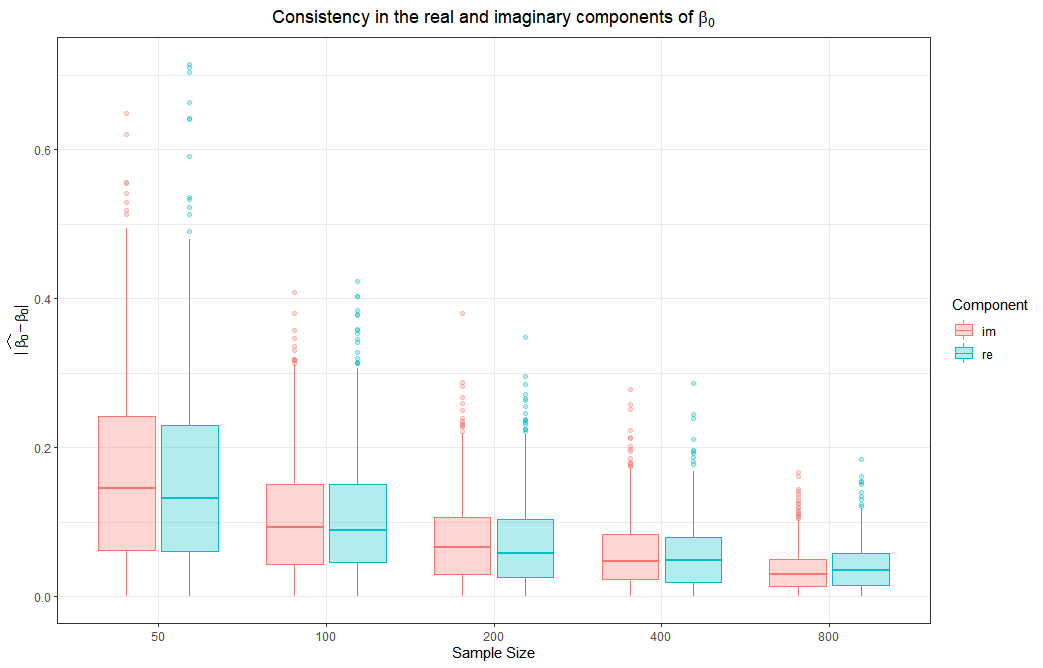
\includegraphics[width = \textwidth]{graphics/CM_consistency_b0_b}
	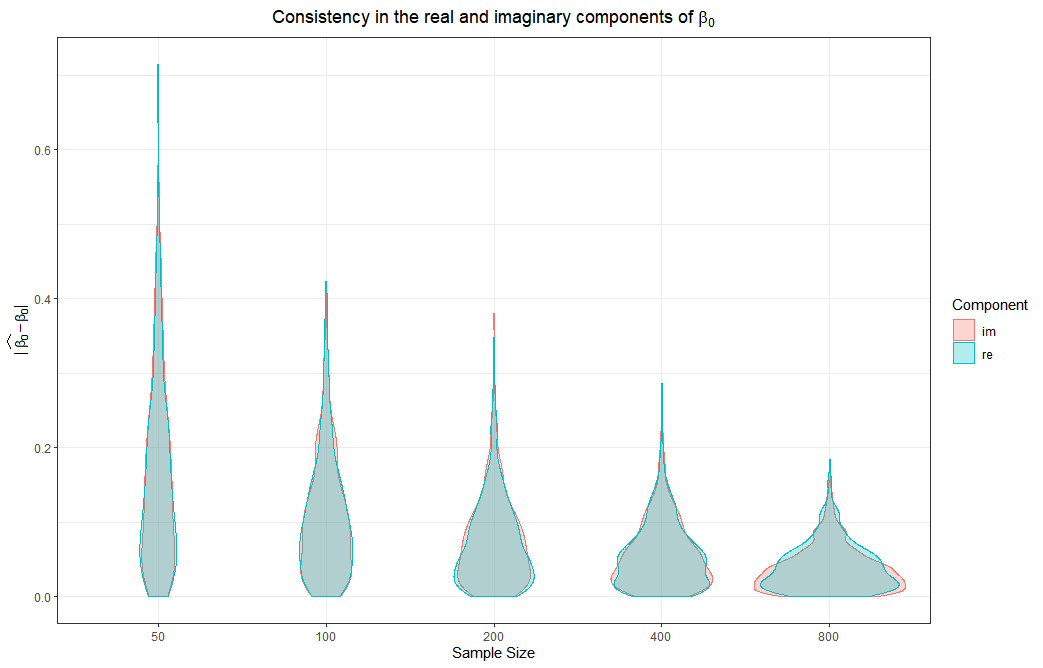
\includegraphics[width = \textwidth]{graphics/CM_consistency_b0_v}
	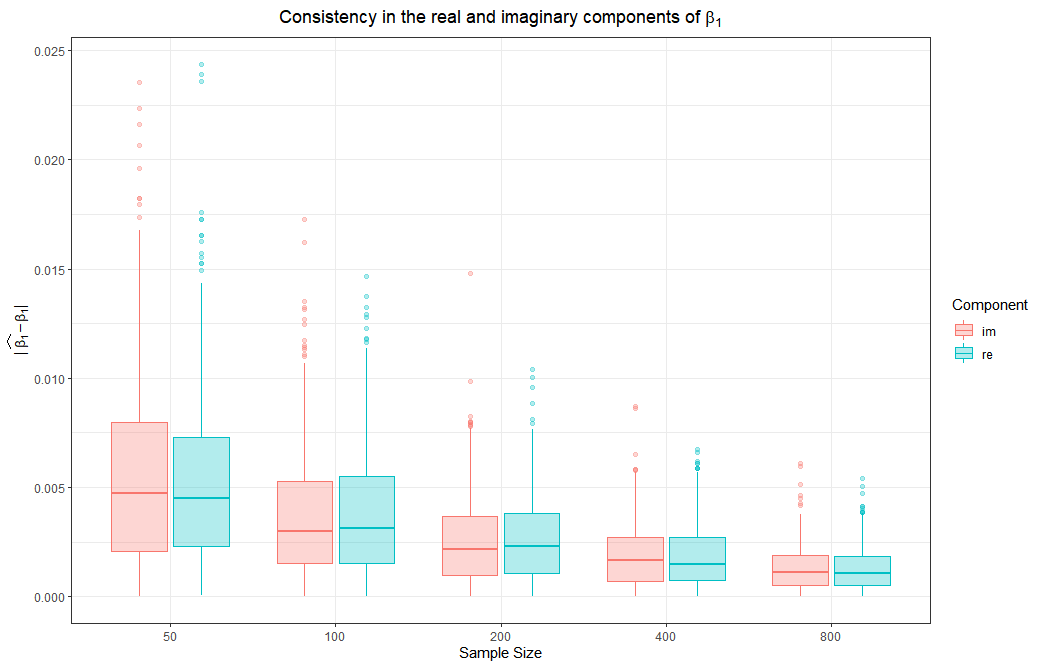
\includegraphics[width = \textwidth]{graphics/CM_consistency_b1_b}
	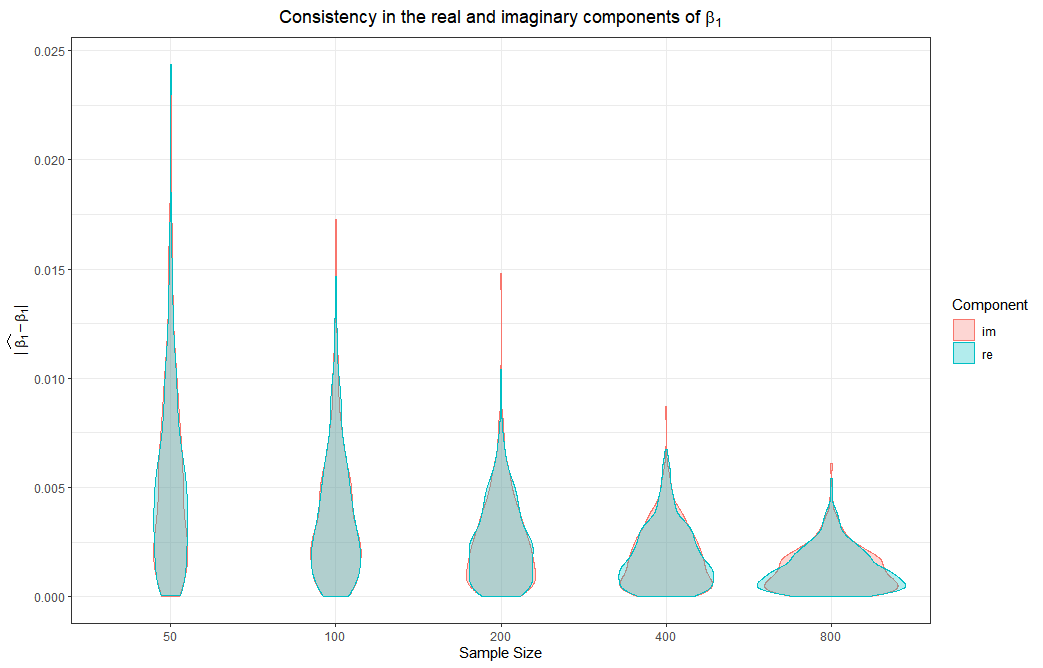
\includegraphics[width = \textwidth]{graphics/CM_consistency_b1_v}
	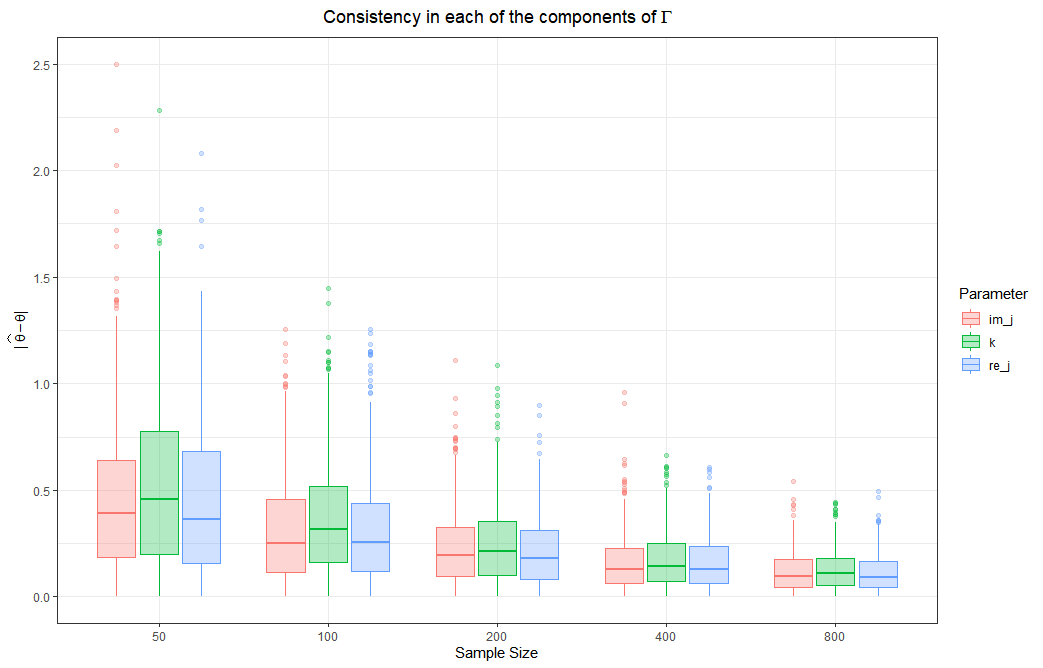
\includegraphics[width = \textwidth]{graphics/CM_consistency_gam_b}
	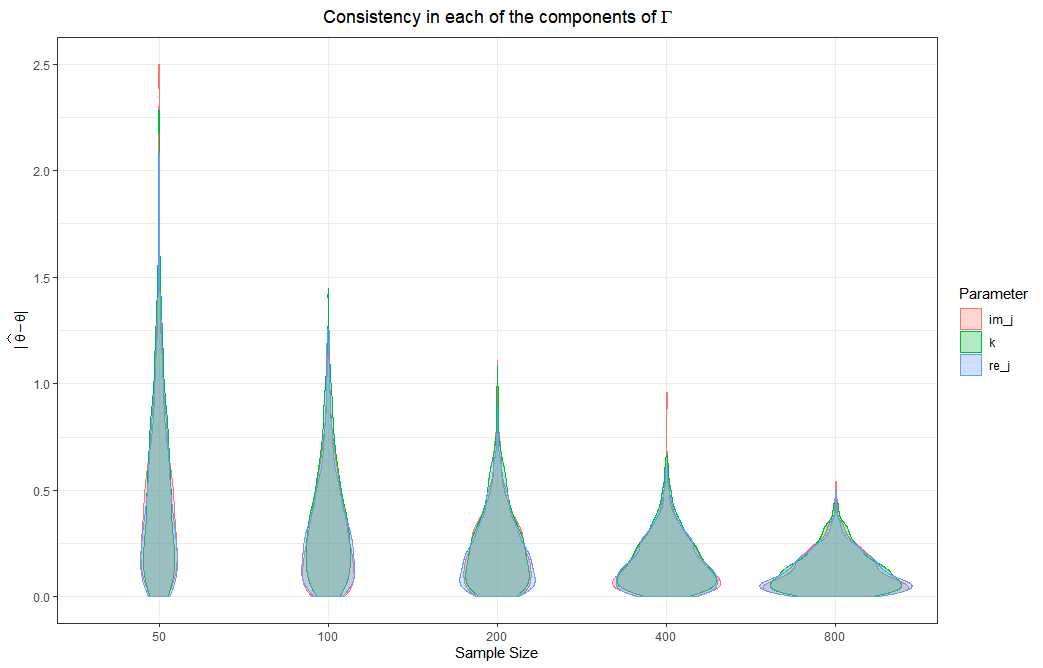
\includegraphics[width = \textwidth]{graphics/CM_consistency_gam_v}
\end{center}

\newpage

%%%%%%%%%%%%%%%%%%%%%%%%%%%%%%%%%%%%%
%%%%%%%%%%%%%%%%%%%%%%%%%%%%%%%%%%%%%
%%%%%%%%%%%%%%%%%%%%%%%%%%%%%%%%%%%%%

\chapter{Simulations}

%%%%%%%%%%%%%%%%%%%%%%%%%%%%%%%%%%%%%

\section{Validating Distributional Properties}

We've shown numerically the consistency of the MLE estimators in the complex regression model in the previous chapter because it lined up better in that section as it paralleled with what was written in \ref{real:consistency}. But now we have the opportunity to show numerically the distributional properties of the regression co-efficients, so that they can be extended for statistical testing.

%%%%%%%%%%%%%%%%%%%%%%%%%%%%%%%%%%%%%

\subsection{Process of Simulating Observations} \label{complex:datagen}

To look at how effective the estimators are and to judge their accuracy compared to other models we must first must know how to simulate from the improper complex normal distribution. Suppose we take the model from \refeq{complexmodel} and take the simplest dimensions where $p = 1$, it becomes a simple complex numbered regression problem, in long form the model will be,

\begin{align*}
	Z_{i} &= \beta_{0} + \beta_{1} x_{i} + \epsilon_{i}.
\end{align*}

\noindent Where $\epsilon_{i} \sim \mathcal{CN} (0, \Gamma)$. The overarching goal is to set some values of $\beta_{0}$ and $\beta_{1}$, randomly generate some observed data $x_{i}$ and draw some $\epsilon_{i} \sim \mathcal{CN} (0, \Gamma)$ to obtain some $Z_{i}$. Then we use the estimators obtained earlier that require the observations $Z_{i}$ and the observed data $x_{i}$ to estimate a $\beta_{0}$ and $\beta_{1}$ eg $\widehat{\beta_{0}}$ and $\widehat{\beta_{1}}$, comparing this with their true values we set at the start. \par

\noindent Getting into more detail, after you have set some regression parameters and have created some observed data, you have to draw some errors from the improper complex normal distribution. To do this we require Definition 1 from Ducharme \cite{ducharme2016}, where if $\bm{\Chi} = (\Chi_{1}, \Chi_{2})^{T} \sim \mathcal{N}_{2} (\mu_{\Chi}, \Sigma_{\Chi})$ and $\Sigma_{\Chi}$ is positive definite, then $Z = \Chi_{1} + j \Chi_{2}$ is complex normally distributed. From here, we can take two approaches to formulate some complex numbered error. Recall the structure of $\Gamma$,

\begin{align*}
	\Gamma &= \begin{pmatrix}
		K & J \\
		J^{*} & K
	\end{pmatrix}.
\end{align*}

\noindent We can choose some $K$ and $J$ such that $\Gamma$ is positive definite and that $K$ is positive because of how it is defined. Or we could choose some parameters for $\Sigma_{\Chi}$ that allow it to be positive definite and that it's diagonals are positive, these two are equivalent and can be determined by one another. For example if $\Gamma$ was defined by the following, then,

\begin{align*}
	\Gamma &= \begin{pmatrix}
		K & \text{Re}(J) + j \text{Im}(J) \\
		\text{Re}(J) - j \text{Im}(J) & K
	\end{pmatrix}, \hspace{1cm}
	\Sigma_{\Chi} = \begin{pmatrix}
		\frac{K + \text{Re}(J)}{2} & -\frac{1}{2} \text{Im}(J) \\
		-\frac{1}{2} \text{Im}(J) & \frac{K - \text{Re}(J)}{2}
	\end{pmatrix}.
\end{align*}

\noindent After those parameters are checked, meaning they will create a positive definite matrix, we then use the ''mvtnorm'' function in R to simulate a pair of observations to serve as the real and imaginary parts of the error, repeating this for however many samples are needed, then combining it all together to create a number of observations that would be distributed $Z_{i} \sim \mathcal{CN} ( \beta_{0} + \beta_{1} x_{i}, \Gamma)$. This is done in our function ''generate\_eps'' in ''simulation\_headers.R'', if you want to check it out.

%%%%%%%%%%%%%%%%%%%%%%%%%%%%%%%%%%%%%

\subsection{Checking the Distribution of the Regression Co-efficients}

We worked out in theory earlier that the regression co-efficients $\widehat{\utilde{\bm{\beta}}}$ are distributed complex normal \refeq{distributionbeta},
\begin{align*}
	\widehat{\utilde{\bm{\beta}}} \sim \utilde{\mathcal{CN}} \left( \utilde{\bm{\beta}}, \left( \sum_{i = 1}^{n} \utilde{x}_{i}^{\ct} \Gamma^{-1} \utilde{x}_{i} \right)^{-1} \right).
\end{align*}

\noindent Using the complex normal property \refeq{CN_property} we discussed earlier we can rearrange this as,

\begin{align*}
	\left( \sum_{i = 1}^{n} \utilde{x}_{i}^{\ct} \Gamma^{-1} \utilde{x}_{i} \right)^{\frac{1}{2}} \left( \widehat{\utilde{\bm{\beta}}} - \utilde{\bm{\beta}} \right) \sim \utilde{\mathcal{CN}} \left( \mathbf{0}, \mathbb{1}_{2p} \right).
\end{align*}

\noindent We can then make an additional transformation into something that is multivariate normally distributed, if we take the matrix $M$ from earlier and give it a $2 p$ by $2 p$ dimensions, we can do the following transformation. Suppose we have a complex normal random vector $\mathbf{Z} \sim \mathcal{CN}(\mathbf{0}, V_{p})$, that it is length $p$ then the augmentation $\utilde{\mathbf{Z}}$ has dimension $2 p$ and is distributed $\utilde{\mathcal{CN}} ( \mathbf{0}, V_{2p} )$ then recall that $\bm{\Chi} = M \utilde{\mathbf{Z}} \sim \mathcal{N}_{2 p} ( \mathbf{0}, \Sigma_{\Chi})$, where the multivariate covariance $\Sigma_{\Chi}$ is related to $V_{2p}$ by $\Sigma_{\Chi} = M V_{2 p} M^{\ct}$ from \refeq{MVTN_CN_cov}. So if do the following,

\begin{align*}
	M \left( \sum_{i = 1}^{n} \utilde{x}_{i}^{\ct} \Gamma^{-1} \utilde{x}_{i} \right)^{\frac{1}{2}} \left( \widehat{\utilde{\bm{\beta}}} - \utilde{\bm{\beta}} \right) &\sim\mathcal{N}_{2 p} \left( \mathbf{0}, M \mathbb{1}_{2p} M^{\ct} \right),\\
	&\sim \mathcal{N}_{2 p} ( \mathbf{0}, \frac{1}{2} M M^{-1} ),\\
	&\sim \mathcal{N}_{2 p} ( \mathbf{0}, \frac{1}{2}\mathbb{1}_{2 p} ),\\
	\sqrt{2} M \left( \sum_{i = 1}^{n} \utilde{x}_{i}^{\ct} \Gamma^{-1} \utilde{x}_{i} \right)^{\frac{1}{2}} \left( \widehat{\utilde{\bm{\beta}}} - \utilde{\bm{\beta}} \right) &\sim \mathcal{N}_{2 p} ( \mathbf{0}, \mathbb{1}_{2 p} ).
\end{align*}

\noindent This is great, because the covariance of the distribution is identity, meaning that each of the terms on the left are independent standard normal. Each component on the left is a standardised real or imaginary component of beta, but the arrangement might be confusing, the first $p$ components are the real components of $\bm{\beta}$ and the last $p$ are the imaginary components. So we can simulate the whole thing and easily separate the components such that each is standard normal, we'll just show this working with $p = 1$ so a complex model with just intercept $\beta_{0}$ and $\beta_{1}$ and $1000$ samples each with $1000$ data points, using the method described earlier. It must be noted that the computation of the square root of the variance $\left( \sum_{i = 1}^{n} \utilde{x}_{i}^{\ct} \Gamma^{-1} \utilde{x}_{i} \right)^{\frac{1}{2}}$ must be done with singular value decomposition or by a Cholesky decomposition, which is quite taxing on computation, but nevertheless, here is the simulation,

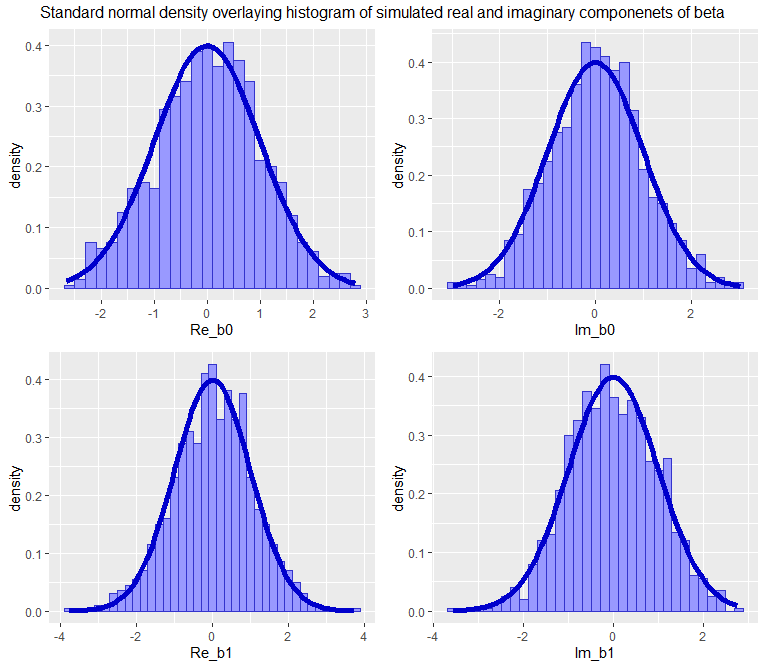
\includegraphics[width = \textwidth]{graphics/samp1000n1000_coloured}

\noindent It looks pretty good, they all seem to follow the standard normal density function pretty nicely and looking at the table of means and standard deviations for each of the components, it looks to confirm our expectations,

\begin{center}
	\begin{tabular}{|c||c|c|c|c|}
	\hline
	& Re$(\beta_{0})$ & Im$(\beta_{0})$ & Re$(\beta_{1})$ & Im$(\beta_{1})$ \\
	\hline \hline
	mean & 0.02960567 & 0.03459596 & 0.01854765 & -0.02643420 \\
	\hline
	sd & 0.9898272 & 0.9694767 & 1.0489810 & 0.9838040 \\
	\hline
	\end{tabular}
\end{center}

\noindent However in practice you would not know the true gamma, you would have to estimate these. We have shown earlier that our gamma estimate converges to the constant true gamma \refeq{gammaconsistent}, demonstrating this further, using the same random seed, we can replace $\Gamma$ with $\widehat{\Gamma}$ in the former simulation of the densities of the components of $\bm{\beta}$ and net the following results,

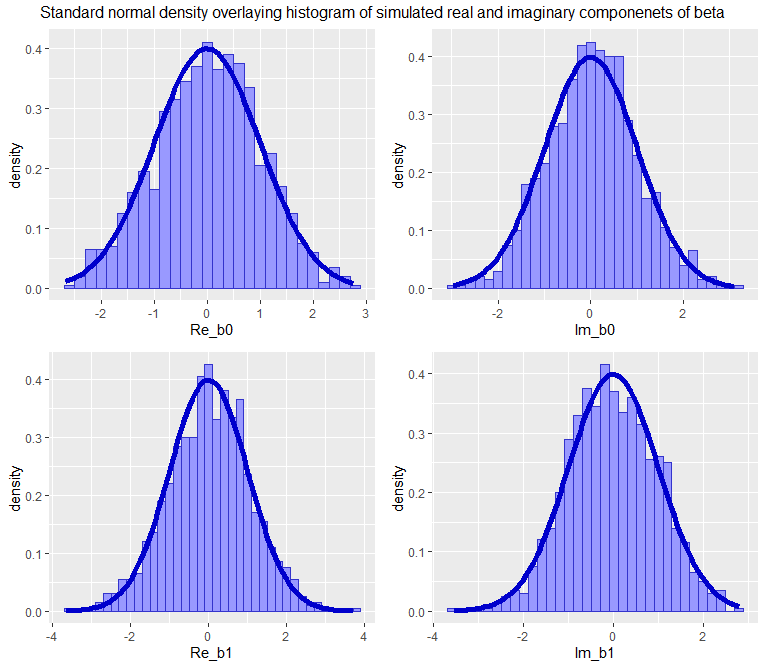
\includegraphics[width = \textwidth]{graphics/density_gamma_est}

\noindent They look so alike! Which is great news as in the upcoming statistical test, we do not have to indulge ourselves in finding $\widehat{\Gamma}$'s awful distribution to test estimates of $\bm{\beta}$. Along with the graphs, we have a similar table,

\begin{center}
	\begin{tabular}{|c||c|c|c|c|}
	\hline
	& Re$(\beta_{0})$ & Im$(\beta_{0})$ & Re$(\beta_{1})$ & Im$(\beta_{1})$ \\
	\hline \hline
	mean & 0.02911989 & 0.03661271 &  0.01876298 & -0.02692299 \\
	\hline
	sd & 0.9893894  & 0.9714519 & 1.0527006 & 0.9864588 \\
	\hline
	\end{tabular}
\end{center}

\noindent When finding the distribution of $\bm{\beta}$ without the known $\Gamma$, but $\widehat{\Gamma}$ we can emplore Slutsky's Theorem, since $\widehat{\utilde{\bm{\beta}}}$ converges in distribution and $\widehat{\Gamma}$ converges in probability we can say,

\begin{align*}
		\sqrt{2} M \left( \sum_{i = 1}^{n} \utilde{x}_{i}^{\ct} \widehat{\Gamma}^{-1} \utilde{x}_{i} \right)^{\frac{1}{2}} \left( \widehat{\utilde{\bm{\beta}}} - \utilde{\bm{\beta}} \right) \xrightarrow{d} \sqrt{2} M \left( \sum_{i = 1}^{n} \utilde{x}_{i}^{\ct} \Gamma^{-1} \utilde{x}_{i} \right)^{\frac{1}{2}} \left( \widehat{\utilde{\bm{\beta}}} - \utilde{\bm{\beta}} \right),
\end{align*}

\noindent where the $d$ denotes in distribution. So we can simply perform z tests on each of the real and imaginary components of $\bm{\beta}$.

%%%%%%%%%%%%%%%%%%%%%%%%%%%%%%%%%%%%%

\subsection{R Code - Iterative Estimation} \label{iterative}

If you note back at \refeq{beta_mle} and \refeq{Kmle} - \refeq{gamma_mle}, the estimate for $\bm{\beta}$ and $\Gamma$ require each other, so to obtain these estimates we must use some numerical method or solve the system of equations. However solving the equations or doing them numerically is extremely convoluted due to large inversion of the $\Gamma$ matrix, so we've come up with a simple yet effective iterative method to compute these inspired by the FGLS method \cite{FGLSwiki}. \par
\noindent The method involves calculating the ordinary least squares estimator for $\bm{\beta}$, then passing it into $\widehat{\Gamma}$, then passing that into the estimator for $\widehat{\utilde{\bm{\beta}}}$ so on and so forth until it converges, depending on the tolerance you set, this converges very quickly, eg at a tolerance $0.0000001$ this generally happens in 3 steps. Because each step requires taking the inverse of a $2 n$ by $2 n$ block diagonal matrix with $2$ by $2$ $\Gamma$ blocks, this does become very costly in computation.

%%%%%%%%%%%%%%%%%%%%%%%%%%%%%%%%%%%%%

\section{Comparisons}

We must check how good our estimator is compared to other linear regression methods on complex numbers, to establish some benefit and then explain why the benefit exists. The two methods we will compare the complex linear regression model with are the method of taking the modulus of the data and running a linear model on that and on a multiple linear regression where the real and imaginary parts are stacked, then the data is regressed on it, however with no specifications on the covariance structure. \par
\noindent Random complex data is going to be generated 1000 times for differing sample sizes and then the three methods will estimate a value for the regression co-efficient $\bm{\beta}$ and their estimates will be compared to the randomly chosen true value.

%%%%%%%%%%%%%%%%%%%%%%%%%%%%%%%%%%%%%

\subsection{Individual Results}

So in the linear model that regresses the modulus of the data, the comparison to the true beta is done by taking the absolute value of the true beta and taking the difference, giving us the following results on the estimates for $\beta_{0}$ and $\beta_{1}$.

\begin{figure}[hpb]
    \centering
    \begin{minipage}{0.5\textwidth}
        \centering
        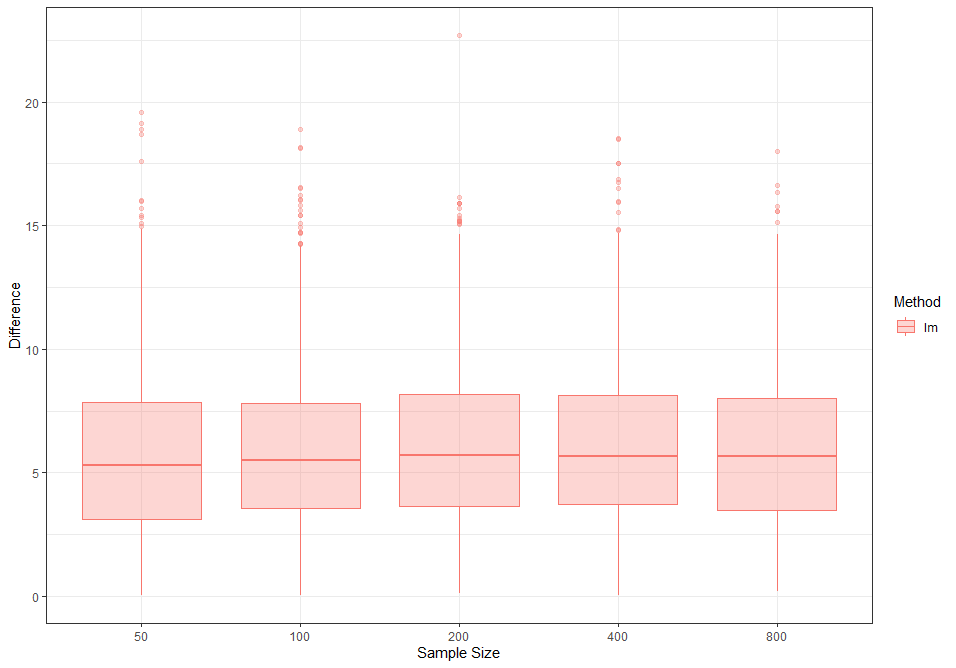
\includegraphics[width=\textwidth]{graphics/b0_lm}
        \caption{Modulus method with $\beta_{0}$}
    \end{minipage}\hfill
    \begin{minipage}{0.5\textwidth}
        \centering
        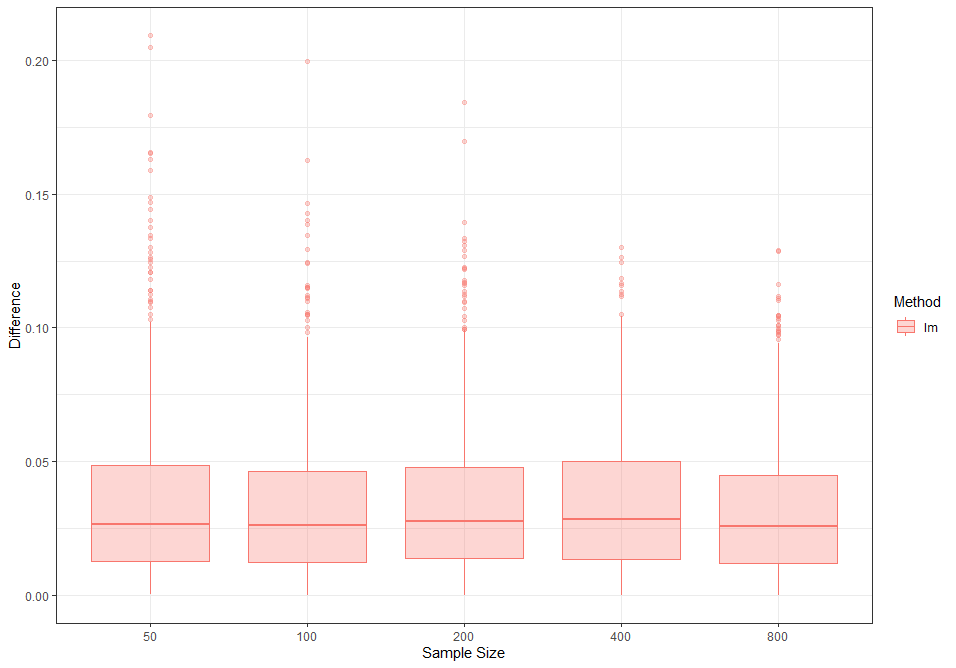
\includegraphics[width=\textwidth]{graphics/b1_lm} 
        \caption{Modulus method with $\beta_{1}$}
    \end{minipage}
\end{figure}

\noindent We see that taking the modulus does not appear to give accurate estimates of $\bm{\beta}$ when it dealing with complex data generated from the complex normal density. The $\beta_{1}$ estimate appears at least close to the true value but neither estimates demonstrate any form of consistency as sample sizes increase.\par

We move on the to multiple linear regression with no specified covariance structure, using the base function ''lm'' in R and regressing the real and imaginary parts of the covariates onto the observations, where the observations are stack real on-top of imaginary.

\begin{figure}[hpb]
    \centering
    \begin{minipage}{0.5\textwidth}
        \centering
        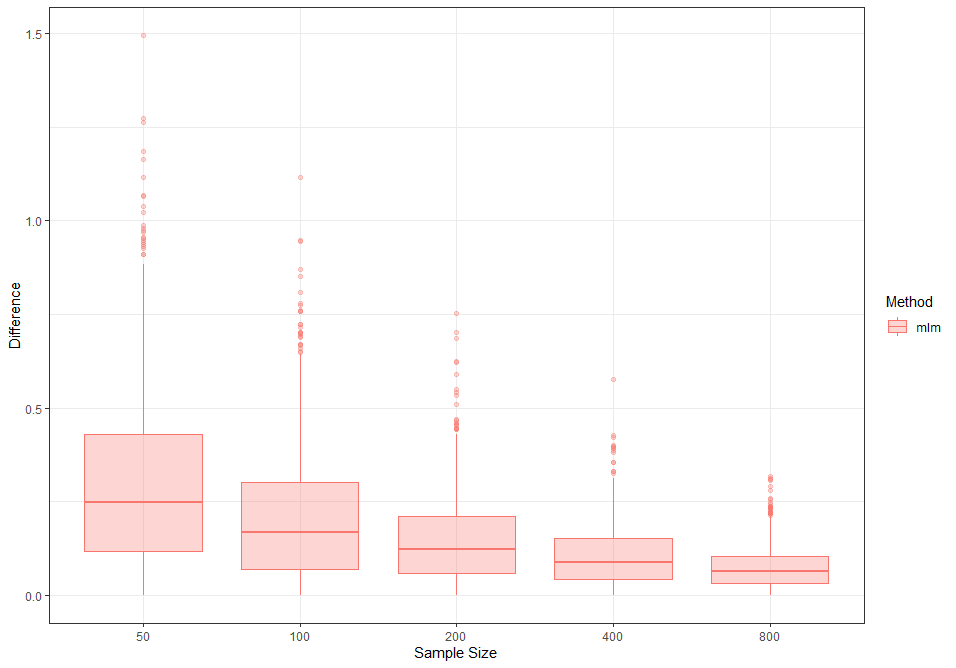
\includegraphics[width=\textwidth]{graphics/b0_mlm}
        \caption{Multivariate method with $\beta_{0}$}
    \end{minipage}\hfill
    \begin{minipage}{0.5\textwidth}
        \centering
        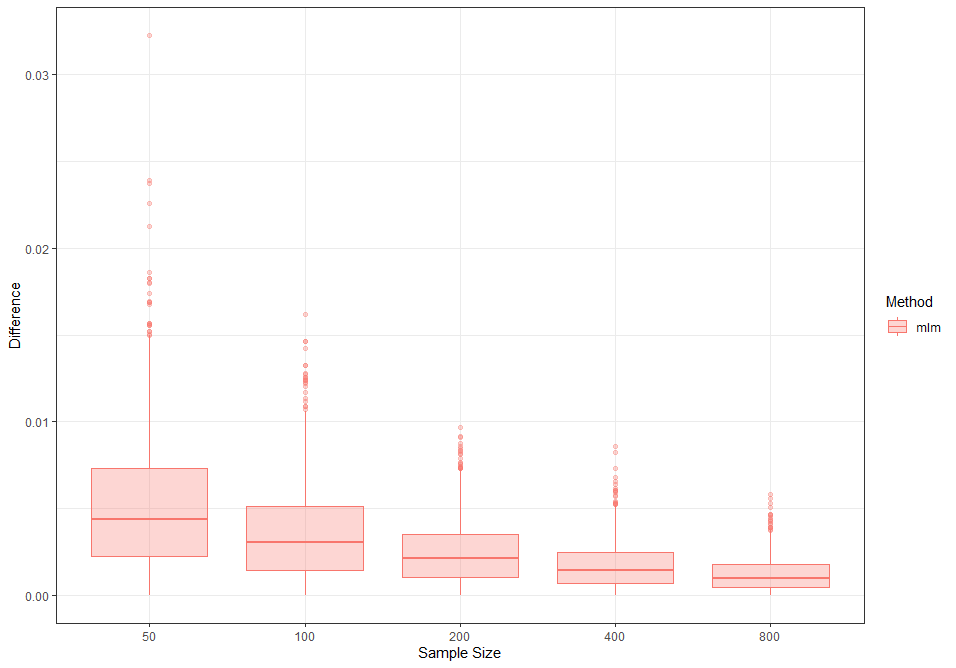
\includegraphics[width=\textwidth]{graphics/b1_mlm} 
        \caption{Multivariate method with $\beta_{1}$}
    \end{minipage}
\end{figure}

\noindent This is more of what we want to see, closeness to the true beta and more accuracy as n increases, similarly we will look at the complex linear regression model.

\begin{figure}[hpb]
    \centering
    \begin{minipage}{0.5\textwidth}
        \centering
        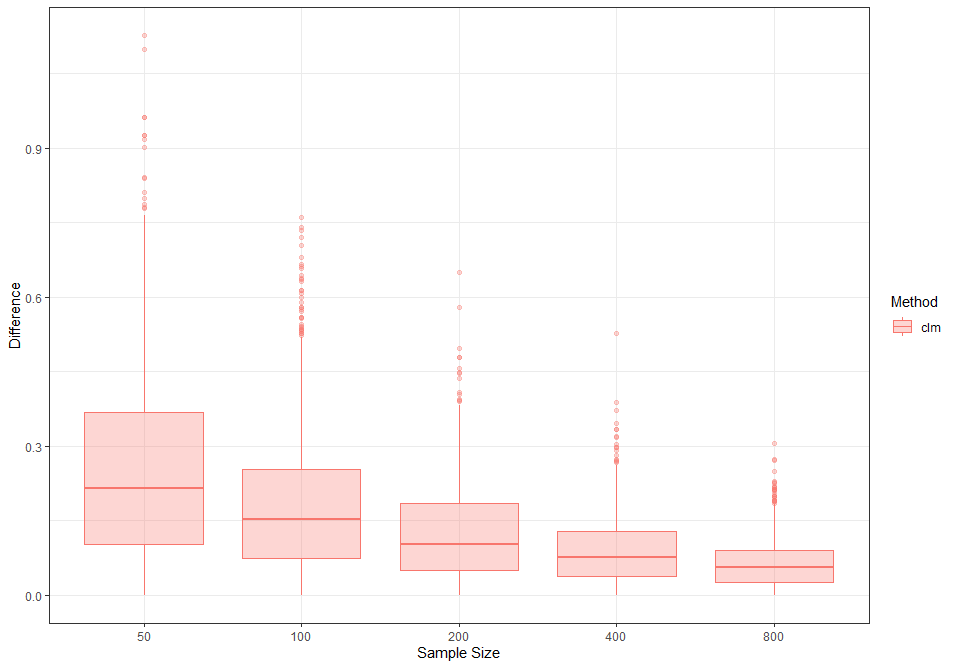
\includegraphics[width=\textwidth]{graphics/b0_clm}
        \caption{Complex method with $\beta_{0}$}
    \end{minipage}\hfill
    \begin{minipage}{0.5\textwidth}
        \centering
        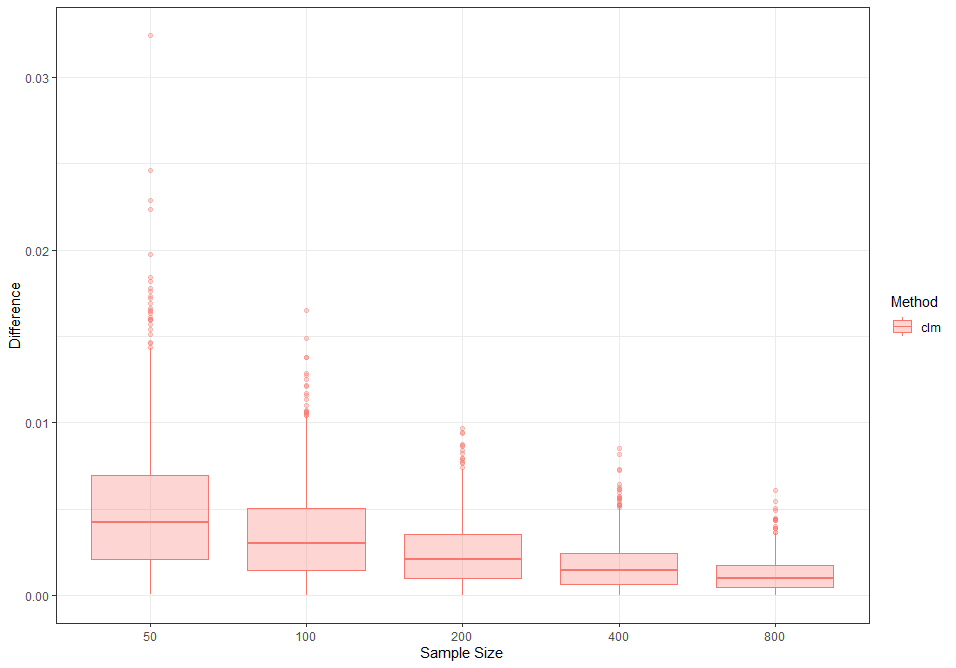
\includegraphics[width=\textwidth]{graphics/b1_clm} 
        \caption{Complex method with $\beta_{1}$}
    \end{minipage}
\end{figure}

\noindent This seems quite similar in property to the multivariate linear model, so we'll check their closeness in the same graph. We will ignore the results of the modulus method, because they were clearly too far from the true values. \par

%%%%%%%%%%%%%%%%%%%%%%%%%%%%%%%%%%%%%

\newpage

\subsection{Side by Side Comparisons}

\begin{figure}[hpb]
    \centering
    \begin{minipage}{0.5\textwidth}
        \centering
        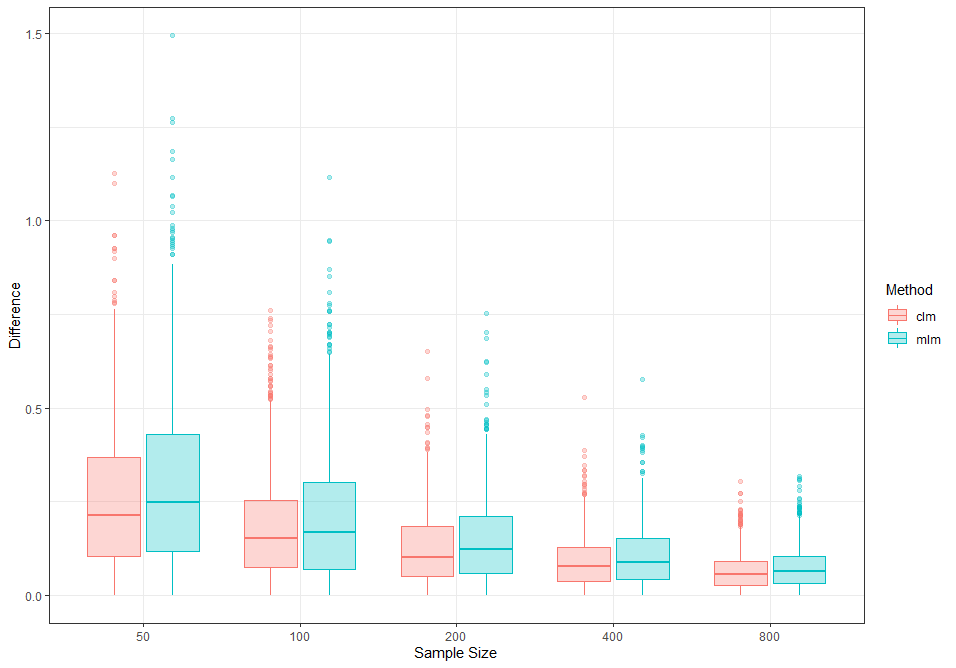
\includegraphics[width=\textwidth]{graphics/b0_clm_mlm}
        \caption{Comparison for $\beta_{0}$}
    \end{minipage}\hfill
    \begin{minipage}{0.5\textwidth}
        \centering
        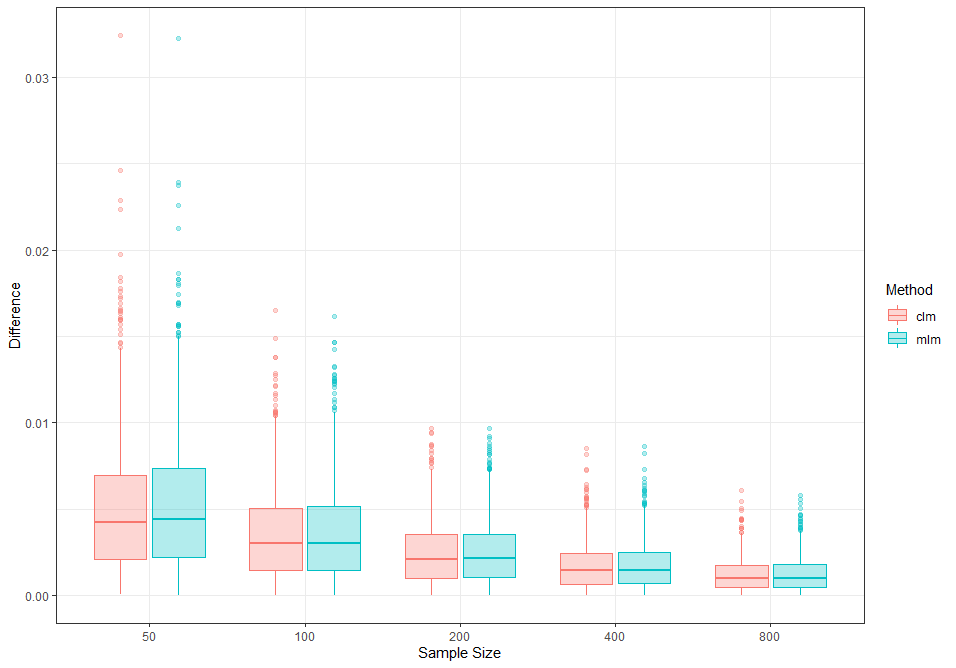
\includegraphics[width=\textwidth]{graphics/b1_clm_mlm} 
        \caption{Comparison for $\beta_{1}$}
    \end{minipage}
\end{figure}

\noindent It is a little hard to see the difference, but complex regression method does better, but not by much especially when considering the $\beta_{1}$ estimate, the complex method is coloured in red (on the left) and the multivariate one in green (on the right). \par

These differences between the two methods really comes down to the specification of covariance structures, because the complex regression model is able to organically describe the variances and covariances of complex normal error by being a specific case of the bi-variate normal distribution and we have taken no specific structure to the covariance structure of the multivariate linear regression method, so it is out performed by the complex one. To get to the same level of accuracy as the complex regression model, a bi-variate covariance structure just be symmetric with different values on the diagonal, none like this was found in the ''gls'' function from the ''nlme'' package \footnote{https://stat.ethz.ch/R-manual/R-devel/library/nlme/html/corClasses.html}.

%%%%%%%%%%%%%%%%%%%%%%%%%%%%%%%%%%%%%
%%%%%%%%%%%%%%%%%%%%%%%%%%%%%%%%%%%%%
%%%%%%%%%%%%%%%%%%%%%%%%%%%%%%%%%%%%%

\chapter{Application - Wind}


We test how effective the method and implementation of complex numbered regression is by applying it to a relatively simple scenario. Here we have wind data, that is a single point in time having wind speed and direction, acting as the modulus and argument of a complex data point. Using past winds (from a day ago) as covariates and current wind as observations. Later on we also introduce time of day and time of year as complex covariates, where the time of day can be measured as a fraction of the total amount of time passed, becoming the argument of a complex number with modulus 1. This makes sense if you imagine a 24 hour clock 00:00 should be right next to 23:59, we do a similar process for time of year.

\section{Introduction to the Problem}

We seek to create value for people who want to model wind for predictive purposes by providing complex regression co-efficients that could have beneficial interpretation and an accurate model for linear regression that can directly intake complex numbered data. The source of the data was introduced earlier, however not the process of acquisition, it was requested from the National Oceanic and Atmosphere Administration and was data from a weather station in Kansas near a town called Coffeyville, the raw data is clean and made usable with perl, all scripts are contained in the github link in the Appendix.

\subsection{Data Cleaning}

The data of course isn't in a perfect state for number crunching immediately most of the work is done by the perl script, ''wind\_script.pl'', extracting the important information from the raw data. Then to create usable complex data,  true bearing must be changed into argument, done by the function ''true\_arg'' in ''simulaton\_headers.R'' and the time covariates are created by passing them as epoch time minus the start of the year. As well as manipulating the data frames to have wind from one day ago or from 30 minutes ago.

\section{Results}

So in a simple case when we regress the wind from the day before hand with the current wind (file ''18\_simulate.R''), taking a sample of 500, we can look at the output of our summary function and at the regression co-efficients.

\newpage

\begin{figure}[h]
	\centering
	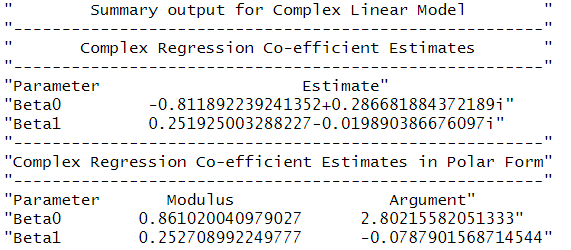
\includegraphics[width = 0.75\textwidth]{graphics/dayBeforeCoef}
	\caption{Summary output for the regressing day before wind on current wind}
\end{figure}

\noindent The output gives two ways to view the regression co-efficients giving more angles to view the problem. These regression co-efficients can be viewed as a sort of intercept and gradient like in the real case, but the interpretation requires more processing. For example ''Beta0'' can be viewed as the current expected wind given that there was no wind the day beforehand, however suppose the wind the day before hand was 10 kilometres an hour northerly, then the current wind would be the vector ''Beta0'' plus the vector ''Beta1'' times $10j$, so the impact of the wind the day before on today's wind is roughly a quarter of the speed it used to be and rotated slightly clockwise. \par

\noindent We also give in the summary output, a printout of the p values of each of the $\beta$ and their real and imaginary components,

\begin{figure}[h]
	\centering
	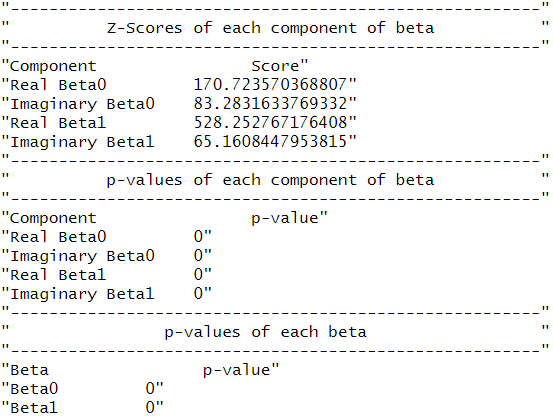
\includegraphics[width = 0.75\textwidth]{graphics/pvals}
	\caption{P-values for the regressing day before wind on current wind}
\end{figure}

\noindent We see because the scores are so large the p-values are going to be 0, due to the limitations in the software, which just means that the wind the day before is significant in forecasting the wind currently.\par

We also introduce the time covariates and see their impact on the model. Practically this can be used to describe winds changing depending on both the time of day and time of year, which in practice does happen, due to winds being changes in pressure and pressure being built from the heating and cooling of the air. So very generally this could help predict where winds would be generally coming from, for a fixed location winds could form a pattern over time due to factors like unique geography, distance from mountain ranges and the sea. 

\begin{figure}[h]
	\centering
	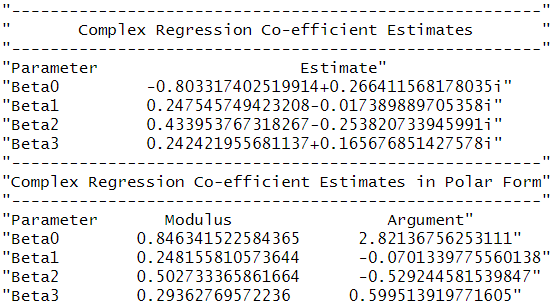
\includegraphics[width = 0.75\textwidth]{graphics/extmodelcoef}
	\caption{P-values for the regressing day before wind on current wind}
\end{figure}

\noindent In this model, ''Beta0'' and ''Beta1'' are the same regression co-efficients as before, however the interpretation of ''Beta2'' is the for the time of day and ''Beta3'' for the time of year, because the two time covariates always have modulus of 1, the interpretation of the model with no previous wind the day before changes. Now it is given a specific time of day and year the expected wind becomes the sum of three vectors, for example for the simplest case, take midnight January 1st, the expected current wind, given no wind the day before becomes the sum of the vectors ''Beta0'',  ''Beta2'' and  ''Beta3''.\par

This could present itself as a different way to run autonomous wind turbines, perhaps where real time methods don't work, the average wind speed and direction could be calculated with covariates like the ones presented in the above model.

% Need to think about what the regression co-efficient for time means
% Better interpretation than a periodic formula Asin(2πh/24)+Bcos(2πh/24) etc
% https://stats.stackexchange.com/questions/164542/is-time-of-the-day-predictor-in-regression-a-categorical-or-a-continuous-varia

%%%%%%%%%%%%%%%%%%%%%%%%%%%%%%%%%%%%%
%%%%%%%%%%%%%%%%%%%%%%%%%%%%%%%%%%%%%
%%%%%%%%%%%%%%%%%%%%%%%%%%%%%%%%%%%%%

\chapter{Conclusion}\label{ccl}

\section{Summary}

The largest take away from this, is the complex regression model being a transformation of the bivariate normal. So the results could potentially be achieved through specific and careful implementation of a bivariate normal model (discussed at the end of Chapter 4). However, we are providing a statistical tool that doesn't require the specific formulation of covariance structure, but naturally accounts for the complex normal noise. In beating out commonly used linear regression tools for complex data, the tool exists as a better method without the difficulty in creating a specific covariance structure.\par
There is the intrinsic value of finding out for completeness that the extension into complex numbers, gives very similar results to the estimators of generalised least squares, however also as the platform to further research, more complicated regression methods and the like. This complex linear regression method also provides a different interpretation into it's regression co-efficients, hence how complex data is related to one another.

\section{Discussion}

There were short comings in this investigation, some due to difficulty, such as the distribution of $\widehat{\Gamma}$ and others due to time, being unable to investigate the convergence of the iterative method \ref{iterative} to calculate the regression parameters. That particular problem also is an avenue to find an exact solution to calculating the maximum likelihood estimates, it seems as though the number of variables and the number of equations match and a non-linear system of equations can be solved. \par
From the very start, a few different regression models could be used, these would potentially lead to different results, one such my co-supervisor had began work on and has suggested that his way has a nicer interpretation of the regression co-efficients. An alternative model was also suggested by my main supervisor, one that look directly at the modulus and argument by splitting the covariate and regression co-efficient into a polar form eg $|\beta_{1}||x_{1}| \exp ( j  \beta_{2} x_{1})$.

%%%%%%%%%%%%%%%%%%%%%%%%%%%%%%%%%%%%%
%%%%%%%%%%%%%%%%%%%%%%%%%%%%%%%%%%%%%
%%%%%%%%%%%%%%%%%%%%%%%%%%%%%%%%%%%%%%%%%%%%%%%%%%%%%%%%%%%%%%%%%%%%%%%%%%

\clearpage
\addcontentsline{toc}{chapter}{References}
\bibliographystyle{unswthesis}

\begin{thebibliography}{999}

\bibitem
{lai1997} Lai, S., Glover, G.H.
Detection of BOLD fMRI signals using complex data,
\textit{Proceedings of the ISMRM} (1997), 1671

\bibitem %1
{rowe2004} Rowe, D.B. and Logan, B.R,
A complex way to compute fMRI activation,
\textit{NeuroImage} \textbf{23} (2004),1078--1092

\bibitem
{picinobo1998} Picinobo, B,
Second-Order Complex Random Vectors and Normal Distributions.,
\textit{IEEE Transactions on Signal Processing, Institute of Electrical and Electronics Engineers} \textbf{44} (1996), 2637--2640

\bibitem %10
{complexstackex} Adrián Barquero, Qiaochu Yuan and Math Stack Exchange community,
Interesting results easily achieved using complex numbers,
\textit{Mathematics Stack Exchange} (2010)

\bibitem
{garcia2011} García-Martín, J., Gómez-Gil, J., Vázquez-Sánchez, E.,
Non-Destructive Techniques Based on Eddy Current Testing,
\textit{Sensors} \textbf{11} (2011), 2525--2565

\bibitem
{yan2012} Yan, C. J., Zhang, S. G. and Ning, W.,
Estimations of the improper linear regression models with complex-valued data,
\textit{Journal of Graduate University of China Academy of Sciences} \textbf{29(2)} (2012), 145--153

\bibitem %14
{mandic2009} Mandic, D.P., Javidi, S., Goh, S.L., Kuh, A., Aihara, K.,
Complex-valued prediction of wind profile using augmented complex statistics,
\textit{Renewable Energy} \textbf{34} (2009), 196--201

\bibitem 
{ducharme2016} Ducharme, G.R., Lafaye de Micheaux, P. and Marchina, B.,
The complex multinormal distribution, quadratic forms in complex random vectors 
and an omnibus goodness-of-fit test for the complex normal distribution,
\textit{Ann Inst Stat Math} \textbf{68} (2016), 77--104

\bibitem
{fischer2002} Fischer, R. F. H.,
Precoding and Signal Shaping for Digital Transmission: Appendix A: Wirtinger Calculus,
\textit{Wiley Online Library} \textbf{A.3.1} 411,
\url{https://onlinelibrary.wiley.com/doi/pdf/10.1002/0471439002.app1}

\bibitem
{wikicomplexnorm} Wikipedia Contributors,
Complex normal distribution --- {Wikipedia}{,} The Free Encyclopedia,
\textit{Wikipedia} (2019),
\url{https://en.wikipedia.org/w/index.php?title=Complex_normal_distribution&oldid=907253384},
[Online; accessed 13-November-2019]

\bibitem
{FGLSwiki} Wikipedia Contributors,
Feasible generalized least squares --- {Wikipedia}{,} The Free Encyclopedia,
\textit{Wikipedia} (2019),
\url{https://en.wikipedia.org/wiki/Generalized_least_squares#Feasible_generalized_least_squares},
[Online; accessed 13-November-2019]


\end{thebibliography}

\begin{appendices}

\chapter{GitHub Link}

\url{https://github.com/jjlt/thesis_files}

\section{File Descriptions}

This file is also found in the github link, it contains a description of the contents of the repository.

\verbatiminput{README.txt}

\end{appendices}

\end{document}





